\documentclass[
	pdftex,%              PDFTex verwenden
	a4paper,%             A4 Papier
	oneside,%             Einseitig
	headsepline,%         Linie nach Kopfzeile
	10pt%                 Gr�ssere Schrift, besser lesbar am bildschrim
]{article}

%
% Paket fuer Uebersetzungen ins Deutsche
%



\usepackage[utf8]{inputenc} % fuer Windows

%
% Paket fuer Quotes
%
\usepackage[babel,french=guillemets,german=swiss]{csquotes}

%
% Paket zum Erweitern der Tabelleneigenschaften
%
\usepackage{array}

%
% Paket fuer schoenere Tabellen
%
\usepackage{booktabs}

%
% Paket um Grafiken einbetten zu koennen
%
\usepackage{graphicx}

\usepackage{scrpage2}
\pagestyle{scrheadings}
% Inhalt bis Section rechts und Chapter links
\automark[section]{chapter}
% Mitte: leer
\chead{}

%
% mathematische symbole aus dem AMS Paket.
%
\usepackage{amsmath}
\usepackage{amssymb}

%
% Type 1 Fonts f�r bessere darstellung in PDF verwenden.
%
%\usepackage{mathptmx}           % Times + passende Mathefonts
%\usepackage[scaled=.92]{helvet} % skalierte Helvetica als \sfdefault
\usepackage{courier}            % Courier als \ttdefault

%
% Paket um Textteile drehen zu k�nnen
%
\usepackage{rotating}

%
% Paket fuer Farben im PDF
%
\usepackage{color}

%
% Paket f�r Links innerhalb des PDF Dokuments
%
\definecolor{LinkColor}{rgb}{0,0,0.5}
\usepackage[%
	pdftitle={Titel},% Titel der Diplomarbeit
	pdfauthor={Autor},% Autor(en)
	pdfcreator={LaTeX, LaTeX with hyperref and KOMA-Script},% Genutzte Programme
	pdfsubject={Betreff}, % Betreff
	pdfkeywords={Keywords}]{hyperref} % Keywords halt :-)
\hypersetup{colorlinks=true,% Definition der Links im PDF File
	linkcolor=LinkColor,%
	citecolor=LinkColor,%
	filecolor=LinkColor,%
	menucolor=LinkColor,%
	pagecolor=LinkColor,%
	urlcolor=LinkColor}

%
% Paket um LIstings sauber zu formatieren.
%
\usepackage[savemem]{listings}
\lstloadlanguages{TeX}

%
% Listing Definationen f�r PHP Code
%
\definecolor{lbcolor}{rgb}{0.85,0.85,0.85}
\lstset{language=[LaTeX]TeX,
	numbers=left,
	stepnumber=1,
	numbersep=5pt,
	numberstyle=\tiny,
	breaklines=true,
	breakautoindent=true,
	postbreak=\space,
	tabsize=2,
	basicstyle=\ttfamily\footnotesize,
	showspaces=false,
	showstringspaces=false,
	extendedchars=true,
	backgroundcolor=\color{lbcolor}}
%
% ---------------------------------------------------------------------------
%


%
% Neue Umgebungen
%
\newenvironment{ListChanges}%
	{\begin{list}{$\diamondsuit$}{}}%
	{\end{list}}

%
% aller Bilder werden im Unterverzeichnis figures gesucht:
%
\graphicspath{{bilder/}}

%
% Literaturverzeichnis-Stil
%
\bibliographystyle{plain}

%
% Anfuehrungsstriche mithilfe von \textss{-anzufuehrendes-}
%
\newcommand{\textss}[1]{"`#1"'}

%
% Strukturiertiefe bis subsubsection{} moeglich
%
\setcounter{secnumdepth}{3}

%
% Dargestellte Strukturiertiefe im Inhaltsverzeichnis
%
\setcounter{tocdepth}{3}

%
% Zeilenabstand wird um den Faktor 1.5 veraendert
%
%\renewcommand{\baselinestretch}{1.5}

%
% Abkuerzungsverzeichnis
%
\usepackage{nomencl}
% Befehl umbenennen in abk
\let\abk\nomenclature
% Deutsche Ueberschrift
\renewcommand{\nomname}{Abk\"urzungsverzeichnis}
% Punkte zw. Abkuerzung und Erklaerung
\setlength{\nomlabelwidth}{.20\hsize}
\renewcommand{\nomlabel}[1]{#1 \dotfill}
% Zeilenabstaende verkleinern
\setlength{\nomitemsep}{-\parsep}
\makenomenclature

\usepackage{eso-pic}
\newcommand\BackgroundPic{%
\put(0,0){%
\parbox[b][\paperheight]{\paperwidth}{%
\vfill
\centering
\includegraphics[width=0.8\paperwidth,height=0.8\paperheight,%
keepaspectratio]{bilder/titelbild.png}%
\vfill
}}}
\usepackage[ngerman]{babel}
\usepackage{pdfpages}
%
% Kapitelueberschriften werden in eine Zeile geschrieben.
%
% normal: 
% Kapitel 1.
% Einleitung
%
% wenn hier auskommentiert:
% Kapitel 1: Einleitung
%
%\usepackage{titlesec}
%\titleformat{\chapter}[hang] 
%{\normalfont\huge\bfseries}{\chaptertitlename\ \thechapter:}{1em}{} 

\begin{document}

\pagenumbering{Roman}

\thispagestyle{empty}

\begin{center}
  %\includegraphics[scale=0.2]{htllogo} \\
  \textbf{\LARGE Administrative Software for Nurseries}
\end{center}
\vspace{10cm}

\begin{flushleft}
\textbf{\LARGE Pflichtenheft}

\vspace{3cm}
\begin{table}[htbp]
\Large
\begin{tabular}{cl}
   Team: & AUKENTALER Lukas \\ 
   & MATTERSBERGER Stefan \\ 
   & MENIA Bernd \\
   & SCHWEIGL Patrik \\
   & STRIEDNIG Emanuel \\
 \end{tabular}
\end{table}
\end{flushleft}

\large Innsbruck, \today

\vfill

\ihead{\leftmark}
\ohead{}
%\input{extras/verzeichnisse}
\newpage
\newcounter{roemisch}
\setcounter{roemisch}{\value{page}}
\pagenumbering{arabic}

%\ihead{\leftmark}
%\ohead{\rightmark}
%\ihead{\parbox[t][2\baselineskip][t]{\dimexpr\linewidth-2em\relax}{\leftmark}}
%\ohead{\parbox[t][2\baselineskip][t]{20em}{\raggedleft\rightmark}}
\tableofcontents
\newpage
\section{System"uberblick}
  Das Ziel dieser Applikation ist es, die administrative Arbeit der Pädagoginnen und Pädagogen von Kinderkrippen zu erleichtern. Unser Fokus liegt dabei auf privaten Kinderstätten, die von Vereinen organisiert und
  finanziert werden. Das System ist zugänglich über eine Login-Plattform für die Mitarbeiter (P"adagogen und Praktikanten) und die Eltern der Kinder (aktiv und inaktiv). Für jeden dieser Akteure werden spezifische Funktionen bereitgestellt.
  Mit unserer Anwendung können die Mitarbeiter Kinder an- und abmelden, Elternteile registrieren, Feiertage und Ferientage verwalten, Kapazit"aten verwalten und die Aufgaben der Eltern eintragen.
 
  Bei den Eltern werden die Akteure weiter unterschieden. Aktive Benutzer sind jene Eltern, die mindestens ein Kind in der Kinderkrippe angemeldet hat. Jene Nutzer k"onnen (alternative) Bring- und Abholzeiten eintragen, diverse
  Abwesenheiten eintragen und das Kind f"urs Essen anmelden.
  
  Unsere Anwendung verf"ugt weiters "uber einen Maildienst, eine Bildergalerie, ein Messageboard und einen privaten Nachrichtendienst, die von den Akteuren verwendet werden k"onnen.
  
\newpage
\section{Use Cases}
  in diesem Kapitel werden die Akteure beschrieben (Kapitel 2.1), das Use-Case-Diagramm wird gezeigt (Kapitel 2.2) und die einzelnen Use Cases werden detailliert beschrieben (Kapitel 2.3 ff.)
  
\subsection{Akteure}
  \subsubsection{Mitarbeiter}
    Unter Mitarbeiter fallen P"adagogen und Praktikanten, die in der Kinderkrippe arbeiten.
    
  \subsubsection{aktiver Elternteil}
    Unter aktiven Elternteilen versteht man Personen, die mindestens ein Kind in der Kinderkrippe angemeldet haben.
    
  \subsubsection{inaktiver Elternteil}
    Unter Inaktive Elternteilen versteht man Personen, deren Kind aus der Kinderkrippe abgemeldet wurde.
    
  \subsubsection{System}  
    
 \newpage
 \subsection{Use-Case-Diagramm}
 \begin{figure}[ht!]
  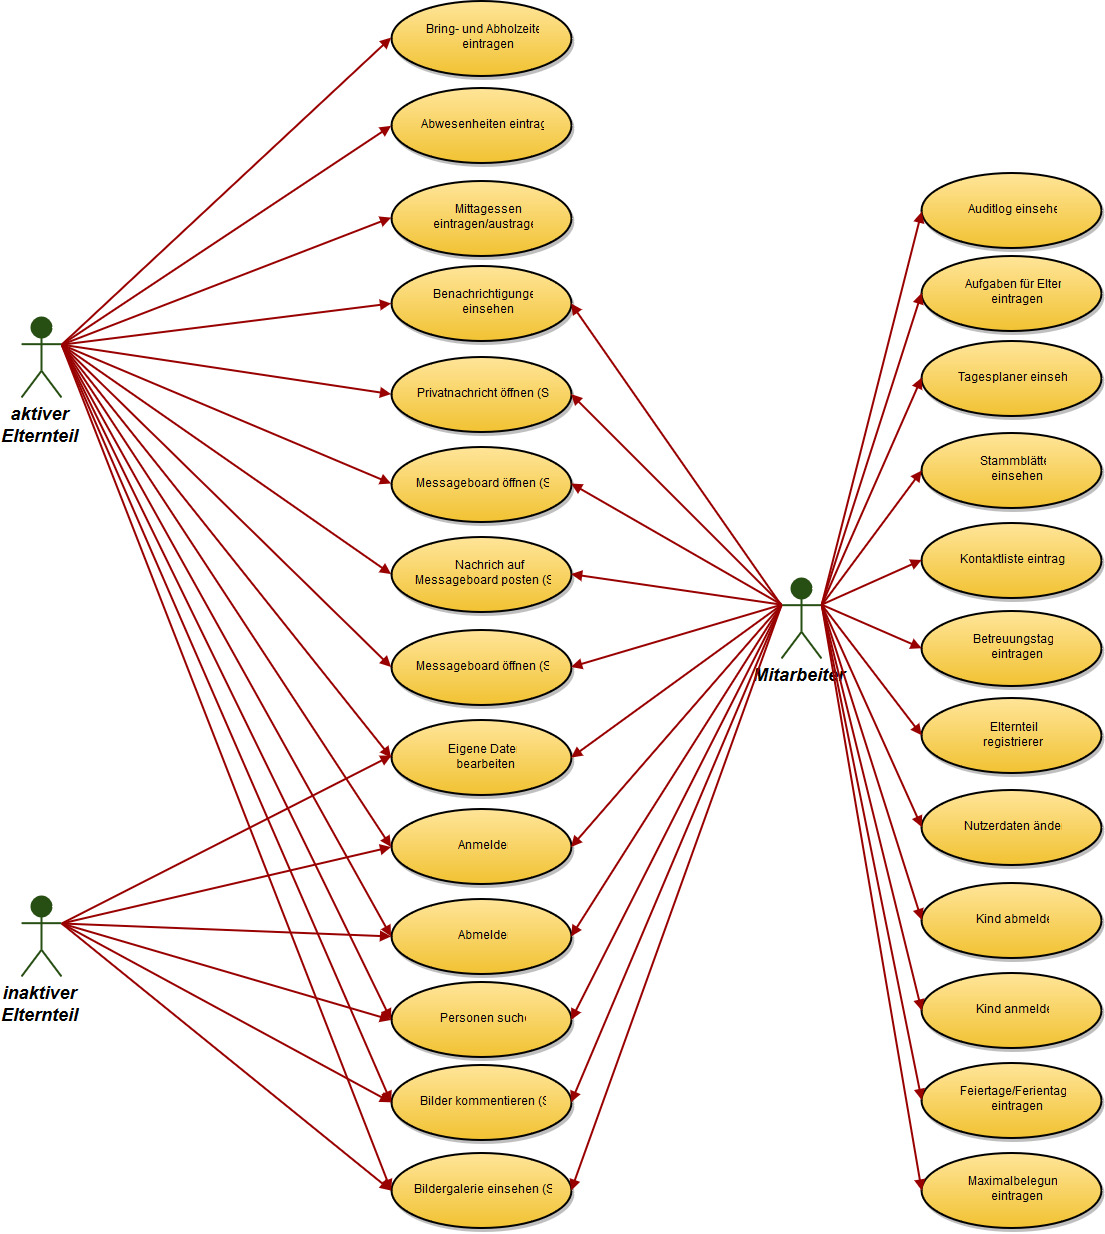
\includegraphics[width = 150mm]{pictures/usecasediagram.jpg}
 \end{figure}

 
 \newpage
 \subsection{Use-Case  Anmelden}
  \paragraph{Identifier}
    UC 2.01
  \paragraph{Beschreibung}
    Um diese Applikation nutzen zu k"onnen, muss sich der Nutzer mit Username und Passwort anmelden.
  \paragraph{Ausl"oser}
    Der Nutzer gibt in den daf"ur vorgesehenen Schaltfl"achen den Benutzernamen und das zugeh"orige Passwort ein und best"atigt seine Eingaben mit dem Button \dq Login \dq.
  \paragraph{Beteiligte Akteure}   \leavevmode \newline
    Mitarbeiter, inaktiver Elternteil, aktiver Elternteil
  \paragraph{Vorbedingungen}
  \begin{itemize}
   \item Es existiert ein g"ultiger Account
   \item Der Nutzer befindet sich in Maske M1-Login
  \end{itemize}

  \paragraph{Schritte}
  \begin{enumerate}
   \item User gibt seinen Username und sein Passwort ein.
   \item Der Benutzer best"atigt seine Eingaben mit dem Button \dq Login\dq
   \item Das System "uberpr"uft die Daten
   \item Der User wird auf die Maske M2-Grundstellung weitergeleitet
  \end{enumerate}

  \paragraph{Alternative Schritte}
  \begin{enumerate}
   \setcounter{enumi}{3}
   \item Die eingegebenen Daten sind nicht korrekt. Der User bekommt eine entsprechende Fehlermeldung
  \end{enumerate}

  \paragraph{Nachbedingungen}
    Der Benutzer befindet sich im angemeldeten Zustand und befindet sich in Maske M2-Grundstellung.

  
 \newpage
 \subsection{Use-Case Abmelden}
  \paragraph{Identifier}
  UC 2.02
  \paragraph{Beschreibung}
  Die aktuelle Sitzung zwischen Benutzer und System wird beendet.
  \paragraph{Ausl"oser}
  \begin{itemize}
   \item Der Benutzer klickt auf den Button \dq Logout\dq
   \item Es hat f"ur einen gewissen Zeitraum keine Eingabe gegeben
   \item Die Applikation wird beendet
  \end{itemize}

  \paragraph{Beteiligte Akteure}   \leavevmode \newline
    Mitarbeiter, inaktiver Elternteil, aktiver Elternteil
  \paragraph{Vorbedingungen}
  \begin{itemize}
   \item Der Benutzer ist angemeldet
  \end{itemize}

  \paragraph{Schritte}
  \begin{enumerate}
   \item Der Benutzer klickt auf den Button \dq Logout\dq
   \item Das System "andert den Status des Benutzers auf \dq abgemeldet\dq
   \item Der Benutzer wird auf die Login Seite M1-Login weitergeleitet
  \end{enumerate}

  \paragraph{Alternative Schritte}
  \begin{enumerate}
  \setcounter{enumi}{0}
   \item Die Applikation wird geschlossen
   \setcounter{enumi}{0}
   \item Der Benutzer hat f"ur eine gewisse Zeit keine Eingabe get"atigt
  \end{enumerate}

  \paragraph{Nachbedingungen}
  Alle aktiven Sitzungen wurden beendet und der Benutzer befindet sich in Maske M1-Login

  
 \newpage
 \subsection{Use-Case Maximalbelegung eintragen}
  \paragraph{Identifier}
  UC 2.03
  \paragraph{Beschreibung}
  Die Mitarbeiter der Kinderkrippe k"onnen nur eine gewisse Anzahl Kinder in Abh"angigkeit der anwesenden P"adagogen und Praktikanten aufnehmen. Diese Anzahl wird gespeichert.
  \paragraph{Ausl"oser}
  Der Mitarbeiter klickt auf den Button \dq Maximalbelegung eintragen\dq
  \paragraph{Beteiligte Akteure}   \leavevmode \newline
    Mitarbeiter
  \paragraph{Vorbedingungen}
  \begin{itemize}
   \item Der Mitarbeiter ist angemeldet
   \item Der Mitarbeiter hat den Rang \dq P"adagoge\dq
  \end{itemize}

  \paragraph{Schritte}
  \begin{enumerate}
   \item Der Mitarbeiter klickt auf den Button \dq Maximalbelegung eintragen\dq
   \item Es "offnet sich ein Pop-up Fenster
   \item Der Benutzer gibt die gew"unschte Anzahl ein und best"atigt mit \dq OK\dq
   \item Die Maximalbelegung wird f"ur den heutigen Tag gespeichert
  \end{enumerate}

  \paragraph{Alternative Schritte}
  \begin{enumerate}
  \setcounter{enumi}{3}
   \item Die Eingabe ist ung"ultig und der Benutzer erh"alt eine entsprechende Fehlermeldung
  \end{enumerate}

  \paragraph{Nachbedingungen}

  
  \newpage
 \subsection{Use-Case Feiertage und Ferienzeiten eintragen}
  \paragraph{Identifier}
  UC 2.04
  \paragraph{Beschreibung}
  Der Mitarbeiter kann Feiertage und kinderkrippenspezifische Ferientage in den Kalender eintragen.
  \paragraph{Ausl"oser}
  Der Mitarbeiter klickt auf den Button \dq Feiertage/Ferien eintragen\dq
  \paragraph{Beteiligte Akteure}   \leavevmode \newline
    Mitarbeiter
  \paragraph{Vorbedingungen}
  \begin{itemize}
   \item der Mitarbeiter ist angemeldet
  \end{itemize}

  \paragraph{Schritte}
  \begin{enumerate}
   \item Der Benutzer klickt auf den Button \dq Feiertage/Ferien eintragen\dq
   \item Der Benutzer wird auf Maske M3-Kalender weitergeleitet
   \item Der Benutzer kann "uber das Kalendermen"u den gew"unschten Tag ausw"ahlen
   \item Es "offnet sich ein Pop-up Fenster
   \item Der Mitarbeiter gibt den gew"unschten Grund und optional eine Anmerkung hinzu
   \item Das System speichert die Daten und der Benutzer wird auf Maske M2-Grundstellung weitergeleitet
  \end{enumerate}

  \paragraph{Alternative Schritte}
  \paragraph{Nachbedingungen}
  Der Feiertag/Ferientag ist f"ur alle auf Makse M3-Kalender sichtbar

  
 \newpage
 \subsection{Use-Case Kind anmelden}
  \paragraph{Identifier}
  UC 2.05
  \paragraph{Beschreibung}
    Die Mitarbeiter k"onnen "uber eine Schaltfl"ache neue Kinder hinzuf"ugen.
  \paragraph{Ausl"oser}
    Der Benutzer klickt auf den Button \dq Kind hinzuf"ugen\dq
  \paragraph{Beteiligte Akteure}   \leavevmode \newline
    Mitarbeiter
  \paragraph{Vorbedingungen}
  \begin{itemize}
   \item Der Mitarbeiter ist angemeldet
   \item Ein Elternteil des Kindes ist registriert
  \end{itemize}

  \paragraph{Schritte}
  \begin{enumerate}
   \item Der Mitarbeiter sucht "uber die Suchfunktion nach dem Elternteil
   \item Der Mitarbeiter w"ahlt das Elternteil aus und akzeptiert die Eingabe.
   \item Der Benutzer klickt auf den Button \dq Kind hinzuf"ugen\dq
   \item Es "offnet sich ein Pop-up Fenster
   \item Der Mitarbeiter gibt alle verpflichtenden Felder ein (Name, Geschlecht, Geburtsdatum, Foto, Notfallkontakt)
   \item Der Mitarbeiter gibt eventuell optionale Felder ein (Allergien, Unvertr"aglichkeiten, Geschwister, sontige Anmerkungen)
   \item Der Mitarbeiter best"atigt seine Eingaben
   \item Das System legt ein neues Kind in der Datenbank an, falls das Elternteil inaktiv war, wird es auf aktiv gesetzt
  \end{enumerate}

  \paragraph{Alternative Schritte}
  \begin{enumerate}
  \setcounter{enumi}{5}
   \item Die eingegeben Daten waren nicht korrekt, dem Benutzer bekommt eine Fehlermeldung
  \end{enumerate}

  \paragraph{Nachbedingungen}
  Der Benutzer befindet sich auf Maske M2-Grundstellung und das Kind befindet sich in der Datenbank

  \newpage
 \subsection{Use-Case Kind abmelden}
  \paragraph{Identifier}
  UC 2.06
  \paragraph{Beschreibung}
  Das Kind kann von der Kinderkrippe abgemeldet werden, wenn das Abmeldedatum "uberschritten wird oder das Personal manuell eine Abmeldung durchf"uhrt.
  \paragraph{Ausl"oser}
  \begin{itemize}
   \item Das Abmeldedatum wird "uberschritten
   \item Das Person meldet das Kind manuell ab
  \end{itemize}

  \paragraph{Beteiligte Akteure}   \leavevmode \newline
    Mitarbeiter
  \paragraph{Vorbedingungen}
  \begin{itemize}
   \item Der Mitarbeiter ist angemeldet
   \item Das Kind ist angemeldet
  \end{itemize}

  \paragraph{Schritte}
  \begin{enumerate}
   \item Der Mitarbeiter such "uber die Suchfunktion das Kind
   \item Der Benutzer best"atigt seine Auswahl
   \item Der Benutzer klickt auf den Button \dq Kind abmleden\dq
   \item Es "offnet sich ein Pop-up Fenster mit einer Abmeldebest"atigung
   \item Der Mitarbeiter best"atigt mit dem Button \dq OK\dq
   \item Das System l"oscht das Kind und alle korrelierten Kontakte, ist kein kind mehr des Elternteils angemeldet, so wird das Elternteil auf inaktiv gesetzt
  \end{enumerate}

  \paragraph{Alternative Schritte}
  \paragraph{Nachbedingungen}
  Der Benutzer befindet sich auf Maske M2-Grundstellung und das Kind wurde abgemeldet

  
  \newpage
 \subsection{Use-Case Benutzerdaten "andern}
  \paragraph{Identifier}
  UC 2.07
  \paragraph{Beschreibung}
  Der Mitarbeiter kann die Daten von Eltern und Kinder "andern oder aktualisieren.
  \paragraph{Ausl"oser}
  Der Mitarbeiter klickt auf den Button \dq Benutzerdaten "andern\dq
  \paragraph{Beteiligte Akteure}   \leavevmode \newline
    Mitarbeiter
  \paragraph{Vorbedingungen}
  \begin{itemize}
   \item Der Mitarbeiter ist angemeldet
   \item Der zu "andernde User ist registriert
  \end{itemize}

  \paragraph{Schritte}
  \begin{enumerate}
   \item Der Mitarbeiter sucht "uber die Suchfunktion die zu "andernde Person
   \item Der Benutzer best"atigt sein Auswahl
   \item Der Benutzer klickt auf den Button \dq Nutzerdaten "andern\dq
   \item Es "offnet sich ein Pop-up Fenster
   \item Der Mitarbeiter "andert die gew"unschten Felder
   \item Der Mitarbeiter best"atigt sine Eingabe
   \item Das System speichert die Daten und wechselt zu Maske M2-Grundstellung
  \end{enumerate}

  \paragraph{Alternative Schritte}
  \begin{enumerate}
  \setcounter{enumi}{4}
   \item Die eingegebenen Daten sind ung"ultig und der Mitarbeiter bekommt eine entsprechende Fehlermeldung
  \end{enumerate}

  \paragraph{Nachbedingungen}
  Die Nutzerdaten wurden ge"andert und der Benutzer befindet sich auf Maske M2-Grundstellung

  
  \newpage
 \subsection{Use-Case Daten drucken}
  \paragraph{Identifier}
  UC 2.08
  \paragraph{Beschreibung}
  Es k"onnen Tagesplaner, Stammbl"atter, Kontaktlisten, Auditlog und Kalender ausgedruckt werden
  \paragraph{Ausl"oser}
    Der Benutzer klickt aud den Button \dq Drucken\dq
  \paragraph{Beteiligte Akteure}   \leavevmode \newline
    Mitarbeiter, inaktiver Elternteil, aktiver Elternteil
  \paragraph{Vorbedingungen}
  \begin{itemize}
   \item Der Benutzer ist angemeldet
   \item Der Benutzer befindet sich in einem der folgenden Masken: M3-Kalender, M4-Auditlog, M5-Tagesplaner, M6-Stammblatt, M7-Kontakte
  \end{itemize}

  \paragraph{Schritte}
  \begin{enumerate}
   \item Der Benutzer klickt auf den Button \dq Drucken \dq
   \item Es "offnet sich ein Pop-up Fenster
   \item Der Benutzer w"ahlt den Drucker aus und best"atigt seine Auswahl
   \item Das System sendet einen Druckerauftrag und wechselt zu M2-Grundstellung
  \end{enumerate}
  \paragraph{Alternative Schritte}
  \paragraph{Nachbedingungen}
  Der Nutzer befindet sich in Maske M2-Grundstellung

  
  \newpage
 \subsection{Use-Case Daten exportieren}
  \paragraph{Identifier}
  UC 2.09
  \paragraph{Beschreibung}
    Es k"onnen Tagesplaner, Stammbl"atter, Kontaktlisten, Auditlog, Kalender und Essensbesllung in CSV/PDF/JSON exportiert werden
  \paragraph{Ausl"oser}
    Der Benutzer klickt aud den Button \dq Daten exportieren\dq

  \paragraph{Beteiligte Akteure}   \leavevmode \newline
    Mitarbeiter, inaktiver Elternteil, aktiver Elternteil
  \paragraph{Vorbedingungen}
    \begin{itemize}
   \item Der Benutzer ist angemeldet
   \item Der Benutzer befindet sich in einem der folgenden Masken: M3-Kalender, M4-Auditlog, M5-Tagesplaner, M6-Stammblatt, M7-Kontakte
  \end{itemize}
  \paragraph{Schritte}
  \begin{enumerate}
   \item Der Benutzer klickt auf den Button \dq Daten exportieren \dq
   \item Es "offnet sich ein Pop-up Fenster
   \item Der Benutzer w"ahlt den das Format und den Speicherort aus und best"atigt seine Auswahl
   \item Das System konvertiert und speichert die Daten und wechselt zu M2-Grundstellung
  \end{enumerate}
  \paragraph{Alternative Schritte}
  \paragraph{Nachbedingungen}
  Der Nutzer befindet sich in Maske M2-Grundstellung

  
  \newpage
 \subsection{Use-Case Elternteil registrieren}
  \paragraph{Identifier}
  UC 2.10
  \paragraph{Beschreibung}
  Wenn ein neues Elternteil dem Verein beitritt, kann es von einem Mitarbeiter registriert werden
  \paragraph{Ausl"oser}
  Der Mitarbeiter klickt auf den Button \dq Elternteil registrieren\dq
  \paragraph{Beteiligte Akteure}   \leavevmode \newline
    Mitarbeiter
  \paragraph{Vorbedingungen}
  \begin{itemize}
   \item Der Mitarbeiter ist angemeldet
  \end{itemize}
  \paragraph{Schritte}
  \begin{enumerate}
   \item Der Benutzer klickt auf den Button \dq Elternteil registrieren\dq
   \item Der Mitarbeiter gibt alle verpflichtenden Felder ein (Name, Geschlecht, Geburtsdatum, Foto)
   \item Der Mitarbeiter best"atigt seine Eingaben
   \item Das System legt einen neuen inaktiven Nutzer an und wechselt zu Maske M2-Grundstellung 
  \end{enumerate}

  \paragraph{Alternative Schritte}
  \begin{enumerate}
  \setcounter{enumi}{1}
   \item Die eingegebenen Daten sind ung"ultig und der Nutzer erh"alt eine Fehlermeldung
  \end{enumerate}

  \paragraph{Nachbedingungen}
  Der neue Nutzer befindet sich in der Datenbank und der Mitarbeiter befindet sich in Maske M2-Grundstellung

  
  \newpage
 \subsection{Use-Case Betreuungstage eintragen}
  \paragraph{Identifier}
  UC 2.11
  \paragraph{Beschreibung}
  Damit die Mitarbeiter wissen, wer an welchem Tag gearbeitet hat, m"ussen Mitarbeiter ihre Betreuungstage eintragen. 
  \paragraph{Ausl"oser}
  Der Mitarbeiter klickt auf den Button \dq Check-in\dq
  \paragraph{Beteiligte Akteure}   \leavevmode \newline
    Mitarbeiter
  \paragraph{Vorbedingungen}
  \begin{itemize}
   \item Der Benutzer ist angemeldet
   \item Der Benutzer befindet sich in M3-Kalender
  \end{itemize}

  \paragraph{Schritte}
  \begin{enumerate}
   \item Der Benutzer klickt in M3-Kalender den gew"unschten Tag
   \item Der Benutzer klickt auf den Button \dq Einchecken\dq
   \item Es "offnet sich ein Pop-up Fenster
   \item Der Benutzer gibt Start- und Endzeit ein
   \item Das System speichert die Daten und der User wird auf M2-GRundstellung weitergeleitet
  \end{enumerate}

  \paragraph{Alternative Schritte}
  \paragraph{Nachbedingungen}
  Die Arbeitszeit wird gespeichert und der User wird auf M2-Grundstellung weitergeleitet
  
  \newpage
  \subsection{Use-Case Kontaktliste einsehen}
  \paragraph{Identifier}
  UC 2.12
  \paragraph{Beschreibung}
  Der Mitarbeiter kann auf eine kompakte Liste mit Namen, Telefonnummer und die angemeldeten Kinder der Eltern zugreifen 
  \paragraph{Ausl"oser}
  Der Mitarbeiter klickt auf den Button \dq Kontaktliste aufrufen\dq
  \paragraph{Beteiligte Akteure}   \leavevmode \newline
    Mitarbeiter
  \paragraph{Vorbedingungen}
  \begin{itemize}
   \item Der Benutzer ist angemeldet
  \end{itemize}

  \paragraph{Schritte}
  \begin{enumerate}
   \item Der Benutzer klickt auf den Button \dq Kontaktliste aufrufen\dq
   \item Das System wechselt zu Maske M7-Kontakte
   \item der Benutzer kann die Kontaktliste "uber Filterfunktionen weiter verfeinern
  \end{enumerate}

  \paragraph{Alternative Schritte}
  \paragraph{Nachbedingungen}
  Der Benutzer befindet sich in M7-Kontakte
  
  
  
	
	\newpage
	\subsection{Use-Case Anlegen von Bezugspersonen}
		\paragraph{Beschreibung}
		Ein Elternteil kann eine Bezugsperson für sein Kind anlegen
		\paragraph{Ausl"oser}
		Der Elternteil klickt auf den Button \dq Bezugsperson hinzuf"ugen\dq
		\paragraph{Beteiligte Akteure}   \leavevmode \newline
		Elternteil
		\paragraph{Vorbedingungen}
			\begin{itemize}
			 	\item Der Elternteil ist angemeldet
			\end{itemize}
		
		\paragraph{Schritte}
			\begin{enumerate}
			 	\item Der Elternteil klickt auf den Button \dq Bezugsperson hinzuf"ugen\dq
			 		\item Es "offnet sich ein Pop-up Fenster in welchem die Daten der Bezugsperson eingetragen werden können
			 	\item Der Elternteil tragt die Daten der Bezugsperson ein
			 	\item Der Elternteil best"atigt die Anlegung mit einem Klick auf den Button "Best"atigen"
			\end{enumerate}
		
		\paragraph{Alternative Schritte}
		Der Elternteil bricht die Anlegung einer Bezugsperson ab. Das Pop-up Fenster wird wieder geschlossen und es werden keine Daten in der Datenbank gespeichert. 	
		\paragraph{Nachbedingungen}
		Die Bezugsperson ist in der Datenbank gespeichert, aber noch nicht im System freigegeben. Die Freischaltung einer Bezugsperson kann daraufhin über einen Mitarbeiter erfolgen. 
		
		
		
	
	\newpage
	\subsection{Use-Case L"oschen von Bezugspersonen (Elternteil)}
	\paragraph{Beschreibung}
		Ein Elternteil kann eine Bezugsperson für sein Kind wieder l"oschen
		\paragraph{Ausl"oser}
		Der Elternteil klickt auf den Button \dq Bezugsperson l"oschen\dq
		\paragraph{Beteiligte Akteure}   \leavevmode \newline
		Elternteil
		\paragraph{Vorbedingungen}
		\begin{itemize}
			\item Der Elternteil ist angemeldet
			\item Mindestens eine Bezugsperson für ein Kind des Elternteils ist in der Kinderkrippe registriert
		\end{itemize}
		
		\paragraph{Schritte}
		\begin{enumerate}
			\item Der Elternteil klickt auf den Button \dq Bezugsperson l"oschen\dq
			\item Es "offnet sich ein Pop-up Fenster in welchem alle Bezugspersonen der Kinder des Elternteils angegeben sind
			\item Der Elternteil w"ahlt eine Bezugsperson aus
			\item Der Elternteil best"atigt den L"oschvorgang mit einem Klick auf den Button "Best"atigen"
		\end{enumerate}
		
		\paragraph{Alternative Schritte}
		Der Elternteil bricht das Löschen einer Bezugsperson ab. Das Pop-up Fenster wird wieder geschlossen und es werden keine Daten in der Datenbank gel"oscht. 	
		\paragraph{Nachbedingungen}
		Die Bezugsperson ist aus der Datenbank entfernt worden. 
  
  
  
  \newpage
  \subsection{Use-Case Kinderstammblatt einsehen (Elternteil)}
  \paragraph{Beschreibung}
  In dieser Ansicht erh"alt der Elternteil die vollst"andigen Information "uber das Kind
  \paragraph{Ausl"oser}
  Der Elternteil klickt auf den Button \dq Kinderstammblatt "offnen\dq
  \paragraph{Beteiligte Akteure}   \leavevmode \newline
  Mitarbeiter
  \paragraph{Vorbedingungen}
  \begin{itemize}
  	\item Der Elternteil ist angemeldet
  	\item Mindestens ein Kind des Elternteils ist in der Kinderkrippe registriert 
  \end{itemize}
  
  \paragraph{Schritte}
  \begin{enumerate}
  	\item Der Elternteil sucht "uber die Suchfunktion sein Kind
  	\item Der Elternteil best"atigt seine Auswahl
  	\item Der Elternteil klickt auf den Button \dq Kinderstammblatt "offnen\dq
  	\item Es "offnet sich ein Pop-up Fenster mit allen Informationen
  \end{enumerate}
	
	\paragraph{Alternative Schritte}
	\paragraph{Nachbedingungen}
	  
    
  
  
  \newpage
 \subsection{Use-Case Kinderstammblatt einsehen (Mitarbeiter)}
  \paragraph{Identifier}
  UC 2.13
  \paragraph{Beschreibung}
  In dieser Ansicht erh"alt der Mitarbeiter die vollst"andigen Information "uber das Kind
  \paragraph{Ausl"oser}
  Der Mitarbeiter klickt auf den Button \dq Kinderstammblatt "offnen\dq
  \paragraph{Beteiligte Akteure}   \leavevmode \newline
    Mitarbeiter
  \paragraph{Vorbedingungen}
  \begin{itemize}
   \item Der Mitarbeiter ist angemeldet
   \item Mindestens ein Kind ist in der Kinderkrippe registriert
  \end{itemize}

  \paragraph{Schritte}
  \begin{enumerate}
   \item Der Mitarbeiter sucht "uber die Suchfunktion das Kind
   \item Der Mitarbeiter best"atigt seine Auswahl
   \item Der Mitarbeiter klickt auf den Button \dq Kinderstammblatt "offnen\dq
   \item Es "offnet sich ein Pop-up Fenster mit allen Informationen
  \end{enumerate}
  
  \paragraph{Alternative Schritte}
  \paragraph{Nachbedingungen}
  
  
  
  
  \newpage
  \subsection{Use-Case Kinderstammblatt bearbeiten (Eltern)}
  \paragraph{Beschreibung}
  Eltern können die Kinderstammblätter ihrer eigenen Kinder bearbeiten. 
  \paragraph{Ausl"oser}
  Der Elternteil klickt auf den Button \dq Kinderstammblatt "offnen\dq
  \paragraph{Beteiligte Akteure}   \leavevmode \newline
  Elternteil
  \paragraph{Vorbedingungen}
  \begin{itemize}
  	\item Der Elternteil ist angemeldet
  	\item Mindestens ein Kind des Elternteils ist in der Kinderkrippe registriert
  \end{itemize}
  
  \paragraph{Schritte}
  \begin{enumerate}
  	\item Der Elternteil sucht "uber die Suchfunktion das Kind
  	\item Der Elternteil best"atigt seine Auswahl
  	\item Der Elternteil klickt auf den Button \dq Kinderstammblatt "offnen\dq
  	\item Es "offnet sich ein Pop-up Fenster mit allen Informationen
  	\item Der Elternteil bearbeitet das Kinderstammblatt
  	\item Der Elternteil schlie"st die Bearbeitung mit einem Klick auf den Button "Best"atigen" ab. 
  \end{enumerate}

  \paragraph{Alternative Schritte}
  \paragraph{Nachbedingungen}
  Die "Anderungen im Kinderstammblatt sind in der Datenbank gespeichert
  
  
  \newpage
  \subsection{Use-Case Kinderstammblatt bearbeiten (Mitarbeiter)}
  \paragraph{Beschreibung}
  Mitarbeiter können die Kinderstammblätter aller Kinder bearbeiten. 
  \paragraph{Ausl"oser}
  Der Mitarbeiter klickt auf den Button \dq Kinderstammblatt "offnen\dq
  \paragraph{Beteiligte Akteure}   \leavevmode \newline
  Mitarbeiter
  \paragraph{Vorbedingungen}
  \begin{itemize}
  	\item Der Mitarbeiter ist angemeldet
  	\item Mindestens ein Kind ist in der Kinderkrippe registriert
  \end{itemize}
  
  \paragraph{Schritte}
  \begin{enumerate}
  	\item Der Mitarbeiter sucht "uber die Suchfunktion das Kind
  	\item Der Mitarbeiter best"atigt seine Auswahl
  	\item Der Mitarbeiter klickt auf den Button \dq Kinderstammblatt "offnen\dq
  	\item Es "offnet sich ein Pop-up Fenster mit allen Informationen
  	\item Der Mitarbeiter bearbeitet das Kinderstammblatt
  	\item Der Mitarbeiter schlie"st die Bearbeitung mit einem Klick auf den Button "Best"atigen" ab. 
  \end{enumerate}
  
  \paragraph{Alternative Schritte}
  \paragraph{Nachbedingungen}
  Die "Anderungen im Kinderstammblatt sind in der Datenbank gespeichert
  
  
  \newpage
 \subsection{Use-Case Tagesplaner einsehen}
  \paragraph{Identifier}
  UC 2.14
  \paragraph{Beschreibung}
  In dieser Ansicht erh"alt der Mitarbeiter eine kompakte "Ubersicht "uber die geplanten T"atigkeiten des gew"ahlten Tages
  \paragraph{Ausl"oser}
  Der Mitarbeiter klickt auf den Button "Tagesplaner einsehen"
  \paragraph{Beteiligte Akteure}   \leavevmode \newline
    Mitarbeiter
  \paragraph{Vorbedingungen}
  \begin{itemize}
   \item Der Benutzer ist angemeldet
   \item Der Benuzer befindet sich in Maske M3-Kalender
  \end{itemize}

  \paragraph{Schritte}
  \begin{enumerate}
   \item Der Benutzer klickt in Maske M3-Kalender auf den gew"unschten Tag
   \item Der Benutzer klickt auf den Button \dq Tagesplaner einsehen\dq
   \item Der Benutzer wird auf die Maske M5-Tagesplaner weitergeleitet
  \end{enumerate}

  \paragraph{Alternative Schritte}
  \paragraph{Nachbedingungen}
  Der Benutzer befindet sich in Maske M5-Tagesplaner

 
 \newpage
 \subsection{Use-Case Aufgaben der Eltern eintragen}
  \paragraph{Identifier}
  UC 2.15
  \paragraph{Beschreibung}
  Die Mitarbeiter der Kinderkrippe k"onnen anfallende Arbeiten Elternteile zuweisen
  \paragraph{Ausl"oser}
  Der Benutzer klickt auf den Button \dq Aufgaben verteilen\dq
  \paragraph{Beteiligte Akteure}   \leavevmode \newline
    Mitarbeiter
  \paragraph{Vorbedingungen}
  \begin{itemize}
   \item Der Benutzer ist angemeldet
   \item Der Benutzer befindet sich in Maske M3-Kalender
   \item Alternativ: Der Benutzer sucht das gew"unschte Elternteil "uber die Suchfunktion
  \end{itemize}

  \paragraph{Schritte}
  \begin{enumerate}
  \item Der Benutzer klickt in Maske M3-Kalender auf den gew"unschten Tag
  \item Der Benutzer klickt auf den Button \dq Aufgaben verteilen\dq
  \item Es "offnet sich ein Pop-up Fenster
  \item der Benutzer gibt alle notwendigen Daten ein (Name, Aufgabe, Zeipunkt, Zeitraum)
  \item Der Benutzer best"atigt seine Eingabe
  \item Das System sendet eine Benachrichtigung an das Elternteil und wechselt zu M2-Grundstellung
  \end{enumerate}
  
  \paragraph{Alternative Schritte}
  \begin{enumerate}
   \item Der Benutzer gibt in die Suchfunktion das gew"unschte Elternteile ein
   \item Der Benutzer klicht auf den Button \dq Aufgabe zuweisen\dq
   \item Es "offnet sich ein Pop-up Fenster
  \item der Benutzer gibt alle notwendigen Daten ein (Name, Aufgabe, Zeipunkt, Zeitraum)
  \item Der Benutzer best"atigt seine Eingabe
  \item Das System sendet eine Benachrichtigung an das Elternteil und wechselt zu M2-Grundstellung
  \end{enumerate}
  \paragraph{Nachbedingungen}
  Das Elternteil erh"alt eine Benachrichtigung und der Nutzer befindet sich in M2-Grundstellung

  
  \newpage
 \subsection{Use-Case Auditlog einsehen}
  \paragraph{Identifier}
  UC 2.16
  \paragraph{Beschreibung}
  Der Auditlog ist eine unver"anderliche Logdatei, die alle Aktionen chronologisch mit Zeitstempel speichert. Auf diese kann "uber unsere Applikation lesend zugegriffen werden 
  \paragraph{Ausl"oser}
  Der Benutzer klickt auf den Button \dq Auditlog lesen\dq
  \paragraph{Beteiligte Akteure}   \leavevmode \newline
    Mitarbeiter
  \paragraph{Vorbedingungen}
  \begin{itemize}
   \item Der Nutzer ist angemeldet
  \end{itemize}

  \paragraph{Schritte}
  \begin{enumerate}
   \item Der Mitarbeiter klickt auf den Button \dq Auditlog lesen\dq
   \item Das System wechselt zur Maske M4-Auditlog
  \end{enumerate}
  \paragraph{Alternative Schritte}
  \paragraph{Nachbedingungen}
  Der Nutzer befindet sich in Maske M4-Auditlog

  
  \newpage
 \subsection{Use-Case Bring- und Abholzeiten eintragen}
  \paragraph{Identifier}
  UC 2.17
  \paragraph{Beschreibung}
  Um den Mitarbeitern die Zeiteinteilung zu erleichtern, k"onnen Eltern die Bring- und Abholzeiten eintragen.
  \paragraph{Ausl"oser}
  Der Benutzer klickt auf den Button \dq Bringen/Abholen\dq
  \paragraph{Beteiligte Akteure}   \leavevmode \newline
    aktiver Elternteil
  \paragraph{Vorbedingungen}
  \begin{itemize}
   \item Der Benutzer ist angemeldet
   \item Der Benutzer befindet sich in Maske M3-Kalender
  \end{itemize}

  \paragraph{Schritte}
  \begin{enumerate}
   \item Der Benutzer klickt in M3-Kalender den gew"unschten Tag an
   \item Der Benutzer klickt auf den Button \dq Bringen/Abholen\dq
   \item Es "offnet sich ein Pop-up Fenster
   \item Der Benutzer gibt die Daten (Bringzeit, Abholzeit, Kind, Selbstabholung oder Fremdabholung) ein und best"atigt seine Eingaben
   \item Das System "uberpr"uft, ob die Bring und Abholzeiten normal oder abweichend sind und markiert sie dementsprechend
   \item Das System speichert die Daten und wechselt zur Maske M2-Grundstellung
  \end{enumerate}

  \paragraph{Alternative Schritte}
  \begin{enumerate}
  \setcounter{enumi}{4}
   \item  Die Eingaben sind ung"ultig und der Benutzer erh"alt eine Fehlermeldung
  \end{enumerate}

  \paragraph{Nachbedingungen}
  Die Bring und Abholzeiten werden in der Datenbank gespeichert und der Nutzer befindet sich in M2-Grundstellung

  
  \newpage
 \subsection{Use-Case Abwesenheit eintragen}
  \paragraph{Identifier}
  UC 2.18
  \paragraph{Beschreibung}
  Der Elternteil kann f"ur das Kind eine au"ssernat"urliche Abwesenheit wie Krankheit oder Arztbesuch eintragen.
  \paragraph{Ausl"oser}
  Der Nutzer klickt auf den Button \dq Abwesenheit eintragen\dq
  \paragraph{Beteiligte Akteure}   \leavevmode \newline
    aktiver Elternteil
  \paragraph{Vorbedingungen}
  \begin{itemize}
   \item Der Benutzer ist angemeldet
   \item Der Benutzer befindet sichin M3-Kalender
  \end{itemize}

  \paragraph{Schritte}
  \begin{enumerate}
   \item Der Benutzer klickt auf M3-Kalender auf den gew"unschten Tag
   \item Der Benutzer klickt auf den Button \dq Abwesenheit eintragen\dq
   \item Es "offnet sich ein Pop-up Fenster
   \item Der Benutzer gibt die erforderlichen Daten (Zeit, Grund) ein und best"atigt seine Eingaben
   \item Das System speichert die Abwesenheit und wechselt zu M2-Grundstellung
  \end{enumerate}

  \paragraph{Alternative Schritte}
  \begin{enumerate}
  \setcounter{enumi}{4}
   \item Die eingegeben Daten sind ung"ultig und der Benutzer erh``alt eine Fehlermeldung
  \end{enumerate}

  \paragraph{Nachbedingungen}
  Der Abwesenheitsgrund wird gespeichert und der Nutzter befindet sich auf M2-Grundstellung

  
  \newpage
 \subsection{Use-Case Mittagessen anmelden/abmelden}
  \paragraph{Identifier}
  UC 2.19
  \paragraph{Beschreibung}
  Das Kind kann w"ochentlich f"ur das Mittagessen angemeldet werden. Eine Abmeldung ist bis zum Stichtag m"oglich.
  \paragraph{Ausl"oser}
  Der Benutzer klickt auf den Button Mitagessen Anmelden/Abmelden
  \paragraph{Beteiligte Akteure}   \leavevmode \newline
    aktiver Elternteil
  \paragraph{Vorbedingungen}
  \begin{itemize}
   \item Der Benutzer ist angemeldet
   \item Der Benutzer befindet sich in M3-Kalender
  \end{itemize}

  \paragraph{Schritte}
  \begin{enumerate}
   \item Der Benutzer klickt in M3-Kalender auf den gew"unschten Tag
   \item Der Benutzer klickt auf den Button \dq Mittagessen Anmelden/Abmelden\dq
   \item Wenn der Benutzer an diesem Tag zu keinem Mittagessen angemeldet ist, "offnet sich ein Pop-up Fenster
   \item Der Benutzer gibt die Wochentage f"ur die folgende Wochen ein, in der das Kind Mittagessen konsumiert
   \item Der Benutzer best"atigt die Eingabe
   \item Das System speichert die Daten und der User wird auf M2-Grundstellung weitergeleitet
  \end{enumerate}

  \paragraph{Alternative Schritte}
  \begin{enumerate}
  \setcounter{enumi}{2}
   \item  Wenn der Benutzer an diesem Tag f"ur ein Mittagessen angemeldet ist, wird die ANmeldung an diesem Tag storniert.
   \item Das System speichert die "Anderung
  \end{enumerate}

  \paragraph{Nachbedingungen}
  Die Anmeldung befindet sich in der Datenbank

  
    \newpage
 \subsection{Use-Case Eigene Daten bearbeiten}
  \paragraph{Identifier}
  UC 2.20
  \paragraph{Beschreibung}
  Die Anwender der Applikation k"onnen jederezeit ihre personenbezogenen Daten "andern
  \paragraph{Ausl"oser}
  Der Benutzer klickt auf den Button \dq Eigene Daten bearbeiten\dq
  \paragraph{Beteiligte Akteure}   \leavevmode \newline
    Mitarbeiter, aktiver Elternteil, inaktiver Benutzer
  \paragraph{Vorbedingungen}
  \begin{itemize}
   \item Der Benutzer ist angemeldet
  \end{itemize}

  \paragraph{Schritte}
  \begin{enumerate}
   \item Der Benutzer klickt auf den Button \dq Eingen Daten bearbeiten\dq
   \item Es "offnet sich ein Pop-up Fenster
   \item Der Benutzer kann seine Daten "andern
   \item Der Benutzer klcikt auf den Button \dq annehmen\dq
   \item Das System speichert die "Anderung und der User wird auf M2-Grundstellung weitergeleitet
  \end{enumerate}

  \paragraph{Alternative Schritte}
  \begin{enumerate}
   \item Die eingegebenen Daten sind ung"ultig und der User erh"alt eine Fehlermeldung
  \end{enumerate}

  \paragraph{Nachbedingungen}
  Der Benutzer befindet sich in M2-Grundstellung

  
  \newpage
 \subsection{Use-Case Benachrichtigungen einsehen und bearbeiten}
  \paragraph{Identifier}
  UC 2.21
  \paragraph{Beschreibung}
  Bei gewissen Aktionen erhalten Benutzer eine Benachrichtigung, die dort angesehen und bearbeitet werden k"onnen
  \paragraph{Ausl"oser}
  Der Benutzer klickt auf den Button \dq Benachrichtigungen\dq
  \paragraph{Beteiligte Akteure}   \leavevmode \newline
    Mitarbeiter, aktiver Elternteil
  \paragraph{Vorbedingungen}
  \begin{itemize}
   \item Der Benutzer ist angemeldet
  \end{itemize}

  \paragraph{Schritte}
  \begin{enumerate}
   \item Der Benutzer klickt auf den Button \dq Benachrichtigungen\dq
   \item Das System wechselt zur Maske M8-Benachrichtigungen
   \item Der Benutzer kann nun die Benachrichtigungen als best"atigt markieren
  \end{enumerate}

  \paragraph{Alternative Schritte}
  \paragraph{Nachbedingungen}

  
  \newpage
 \subsection{Use-Case Messageboard "offnen (Sonderfunktion)}
  \paragraph{Identifier}
  UC 2.22
  \paragraph{Beschreibung}
  Der Benutzer "offnet das Messageboard mit Klick auf einen Button. Es öffnet sich eine Seite mit chronologisch angeordneten Textfeld-Komponenten (Neueste zuerst). 
  \paragraph{Ausl"oser}
  \paragraph{Beteiligte Akteure}   \leavevmode \newline
    Mitarbeiter, aktiver Elternteil
  \paragraph{Vorbedingungen}
  \paragraph{Schritte}
  \paragraph{Alternative Schritte}
  \paragraph{Nachbedingungen}

  
  \newpage
 \subsection{Use-Case Nachricht auf Messageboard posten (Sonderfunktion)}
  \paragraph{Identifier}
  UC 2.23
  \paragraph{Beschreibung}
  Über das Eingabefeld können neue Nachrichten (Textfeld-Komponenten) erstellt werden. Diese Nachricht wird für jeden aktiven Elternteil sichtbar.
  \paragraph{Ausl"oser}
  \paragraph{Beteiligte Akteure}   \leavevmode \newline
    Mitarbeiter, aktiver Elternteil
  \paragraph{Vorbedingungen}
  \paragraph{Schritte}
  \paragraph{Alternative Schritte}
  \paragraph{Nachbedingungen}
  
  \newpage
 \subsection{Use-Case Privatnachricht senden (Sonderfunktion)}
  \paragraph{Identifier}
  UC 2.24
  \paragraph{Beschreibung}
  \paragraph{Ausl"oser}
  \paragraph{Beteiligte Akteure}   \leavevmode \newline
    Mitarbeiter, aktiver Elternteil
  \paragraph{Vorbedingungen}
  \paragraph{Schritte}
  \paragraph{Alternative Schritte}
  \paragraph{Nachbedingungen}

  
  \newpage
 \subsection{Use-Case Bildergalerie "offnen (Sonderfunktion)}
  \paragraph{Identifier}
  UC 2.25
  \paragraph{Beschreibung}
  \paragraph{Ausl"oser}
  \paragraph{Beteiligte Akteure}   \leavevmode \newline
    Mitarbeiter, inaktiver Elternteil, aktiver Elternteil
  \paragraph{Vorbedingungen}
  \paragraph{Schritte}
  \paragraph{Alternative Schritte}
  \paragraph{Nachbedingungen}

  
  \newpage
 \subsection{Use-Case Bilder kommentieren (Sonderfunktion)}
  \paragraph{Identifier}
  UC 2.26
  \paragraph{Beschreibung}
  \paragraph{Ausl"oser}
  \paragraph{Beteiligte Akteure}   \leavevmode \newline
    Mitarbeiter, inaktiver Elternteil, aktiver Elternteil
  \paragraph{Vorbedingungen}
  \paragraph{Schritte}
  \paragraph{Alternative Schritte}
  \paragraph{Nachbedingungen}

  
  \newpage
 \subsection{Use-Case Personen suchen}
  \paragraph{Identifier}
  UC 2.27
  \paragraph{Beschreibung}
  Um die Handhabung mit Personen zu vereinfachen, k"onnen die Benutzer der Anwendung die Personen "uber verschiedene Filterfunktionen suchen
  \paragraph{Ausl"oser}
  Der Benutzer gibt den Namen der Person in die Suchmaske ein
  \paragraph{Beteiligte Akteure}   \leavevmode \newline
    Mitarbeiter, inaktiver Elternteil, aktiver Elternteil
  \paragraph{Vorbedingungen}
  \begin{itemize}
   \item Der Benutzer ist angemeldet
  \end{itemize}

  \paragraph{Schritte}
  \begin{enumerate}
   \item Der Benutzer gibt den Namen in die Suchmaske ein
   \item Das System gibt dynamisch passende Personen zur"uck
  \end{enumerate}

  \paragraph{Alternative Schritte}
  \begin{enumerate}
   \item Der Benutzer klickt bei der Suchmaske auf \dq Filter anwenden\dq
   \item Der Benutzer verwendet die verschiedenen Filter
   \item Das System gibt dynamisch passende Personen zur"uck
  \end{enumerate}

  \paragraph{Nachbedingungen}



\newpage
\section{Klassendiagramm}

 \subsection{Klassendiagramm}
 \begin{figure}[ht!]
  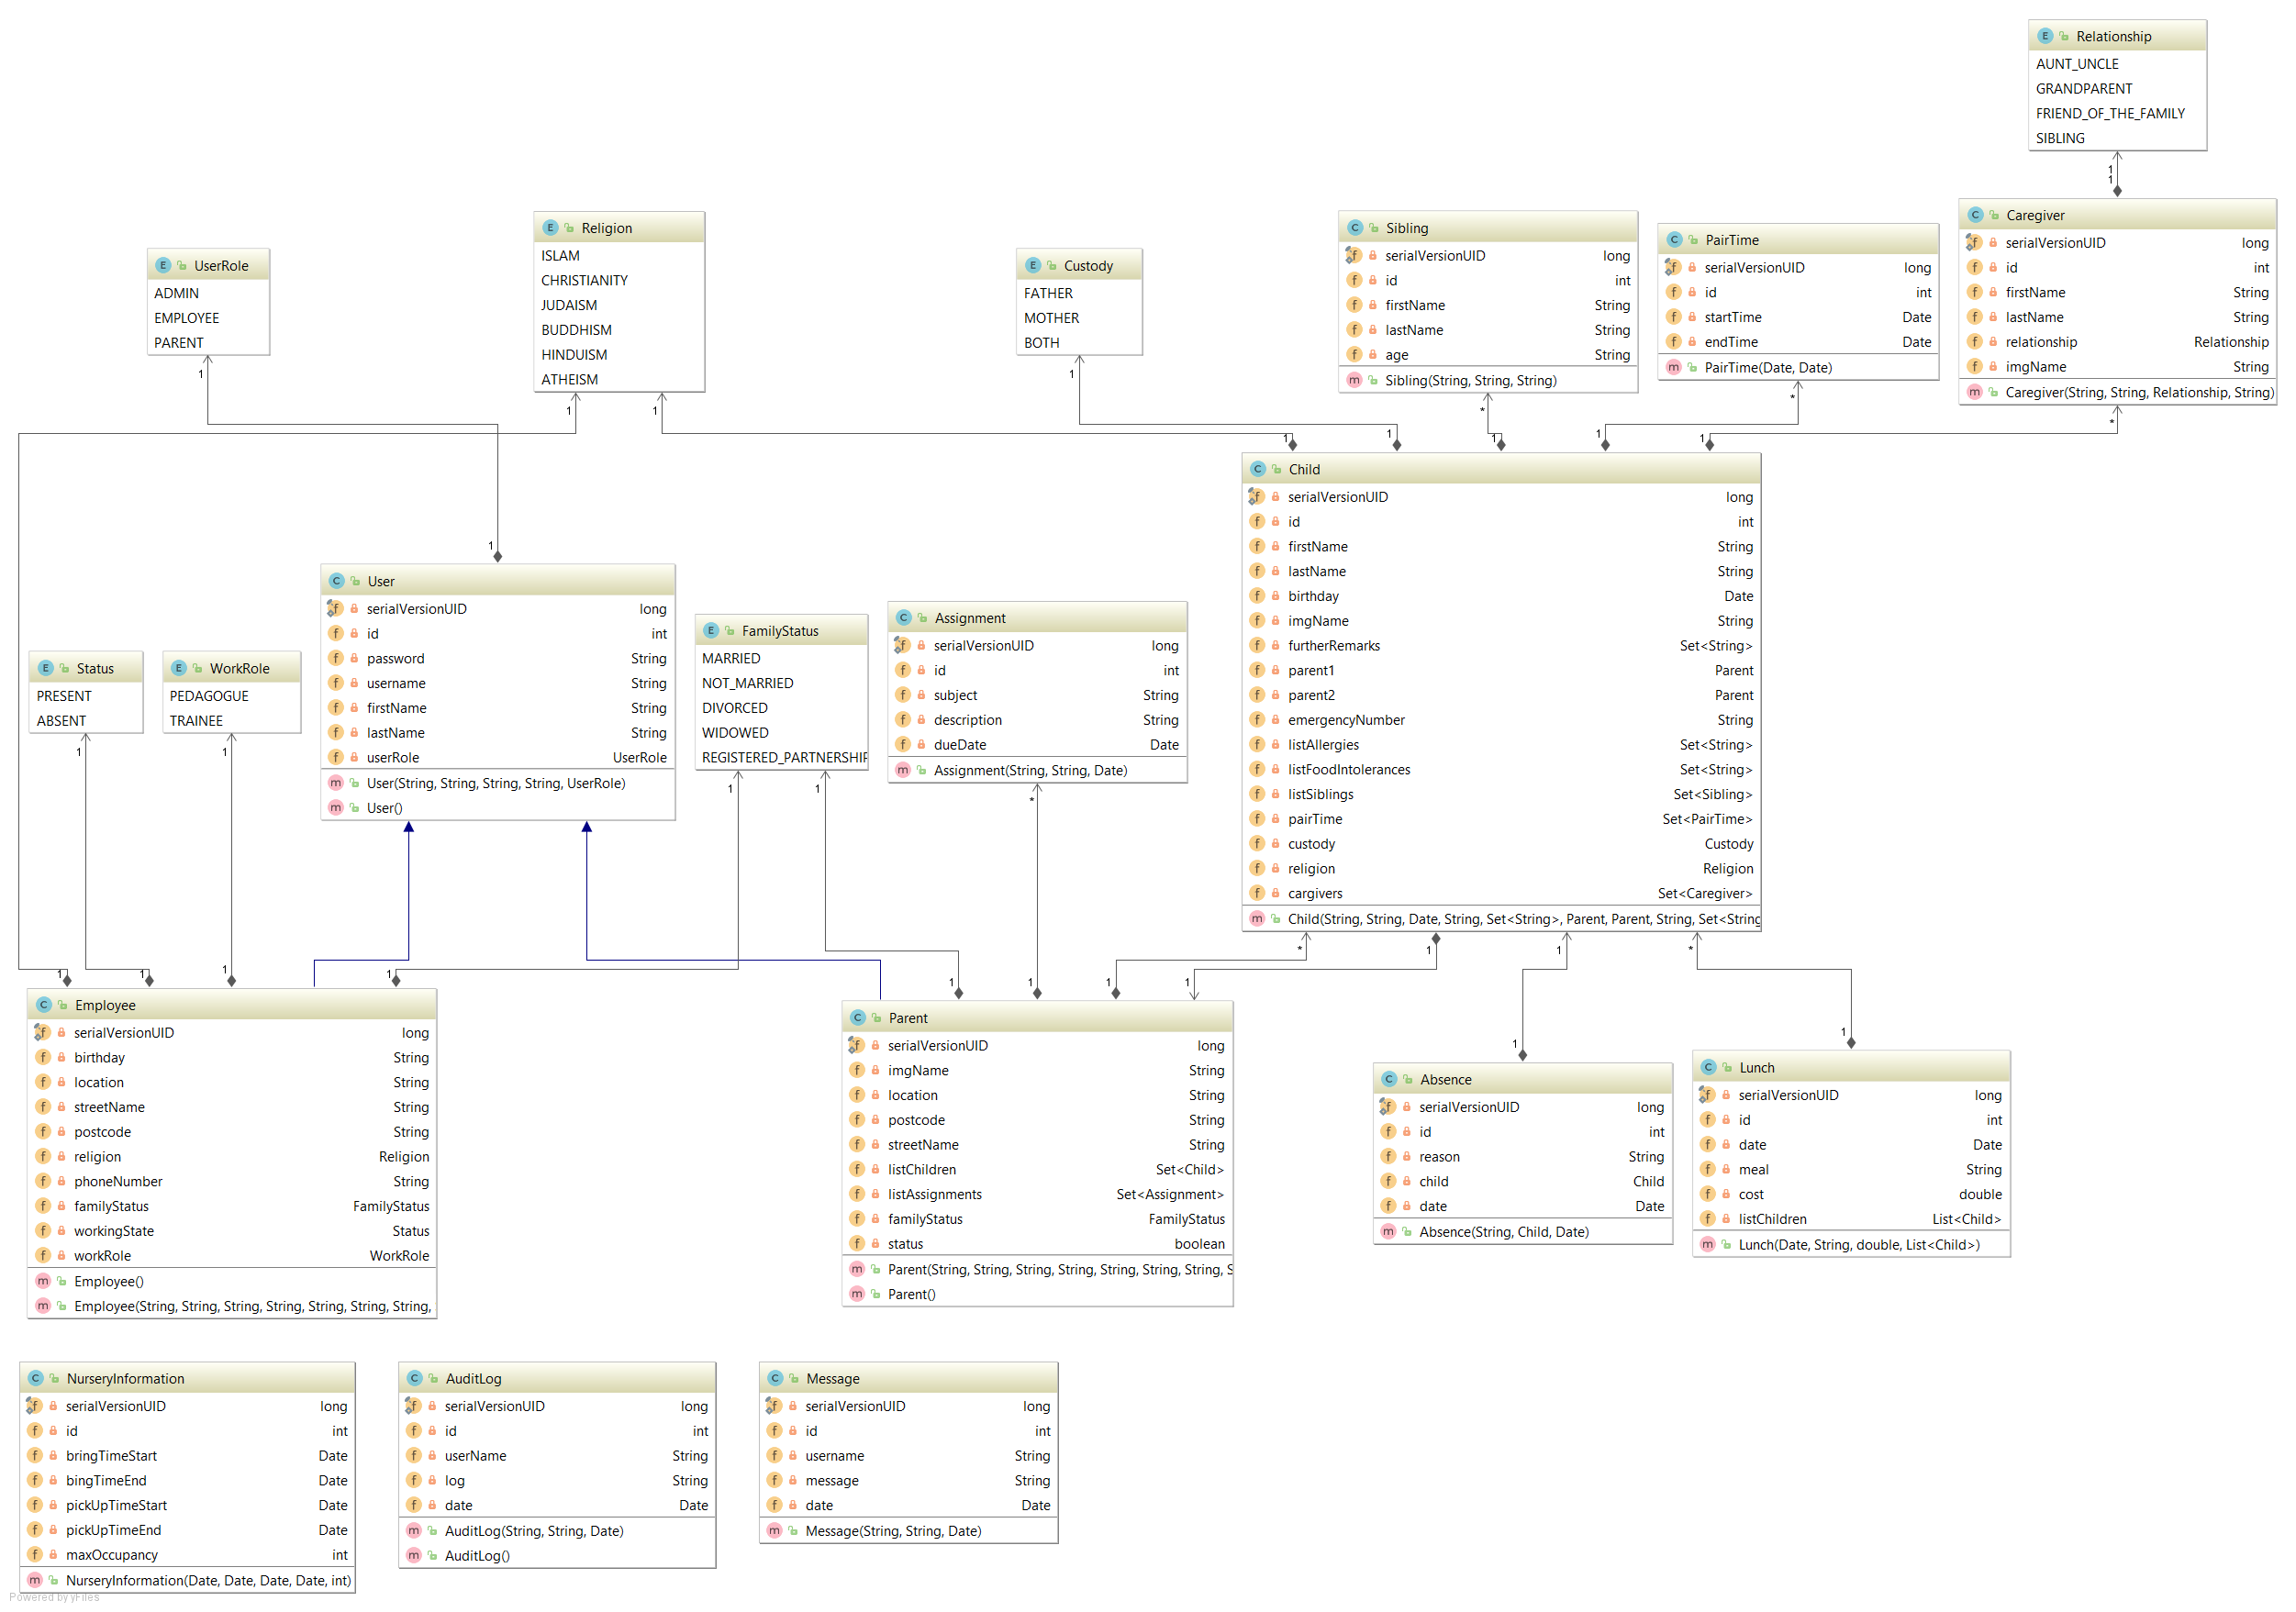
\includegraphics[width = 150mm]{pictures/class_diagram_intellij_bright.png}
 \end{figure}

\newpage
\subsection{Child}
	Haupt-Klasse für alle Kinder die in der Kinderkrippe registriert sind. Zusätzlich zu Attributen wie Namen, Geburtsdatum oder Elternteile sind in dieser Klasse auch Informationen zu Allergien, Nahrungsmittelunverträglichkeiten oder Geschwistern vorhanden. 
\paragraph{Absence}
	Wenn ein Kind an einem regulären Tag von der Kinderkrippe fernbleibt muss dieser Verbleib in dieser Klasse festgehalten werden. Dafür wird der Grund in Form eines Strings abgespeichter und zusätzlich nocht das Kind selber und das Datum der Abwesenheit notiert.
\paragraph{Custody}
	Gibt an welche Elternteile (Vater, Mutter oder beide) für die Obhut eines Kindes verantwortlich sind. 
\paragraph{Pairtime}
	Diese Klasse besteht aus einem Paar von java.util.Date. Wir haben diese Klasse erstellt um zum Beispiel Abhol- und Bringzeiten klar darstellen zu können. 
\paragraph{Sibling}
	Sibling ist eine kleinere Version der Child-Klasse. Jeder Bruder / Schwester ist zwar ebenfalls als Kind in der Kinderkrippe registriert, wird hier aber nur mit dem vollständigen Namen und Alter referenziert um unnötige Datenduplizierung zu vermeiden. 

\subsection{Employee}
	In Employee werden alle Pädagogen und Auszubildene festgehalten. Pädagogen (Enum WorkRole) haben Zugriff auf alle Daten der Kinder und der Auszubildenden. 
\paragraph{Status}
	Beinhaltet Information über An- und Abwesenheit eines Mitarbeiters. 
\paragraph{WorkRole}
	Gibt an ob ein Mitarbeiter ein Pädagoge oder ein Auszubildender ist.
	
\subsection{Nursery}
\paragraph{AuditLog}
	Im AuditLog werden alle Ereignisse gespeichert die Datenbanktechnisch relevant sind. Hierzu gehören erstellen, löschen und editieren von Benutzern. Jeder Eintrag im AuditLog wird mit einer timestamp und dem Benutzer versehen, welcher den Eintrag hervorgerufen hat. 
\paragraph{Lunch}
	Speichert alle nötigen Werte für das tägliche Mittagessen, zu dem die Eltern ihre Kinder anmelden können. Es werden Datum, Mahlzeit, Kosten und die Liste der angemoldenen Kinder vermerkt. Sowohl Mitarbeiter als auch Eltern haben Zugriff auf diese Klasse, wobei nur Mitarbeiter die Werte verändern können.
\paragraph{Message}
	Benutzer können im Messageboard Nachrichten erstellen. Um dies zu ermöglichen verwenden wir "Message" als Hilfsklasse. 
\paragraph{NurseryInformation}
	NurseryInformation beinhaltet die Zeiten an denen Eltern ihre Kinder in die Kinderkrippe bringen und wieder abholen können. Zudem wird noch ein Wert abgespeichert, der die Maximalbelegung der Kinderkrippe anzeigt. 
	
\subsection{User}
User ist die Ausgangsklasse für die Klassen Employee und Parent. Sie bietet grundlegende Attribute wie etwa userName, password, firstName, lastName und die userRole. 
In unserer Implementierung ist ein Admin vorhanden, jedoch nicht als eigene Klasse, da wir Datenbanktechnisch in einige Probleme liefen. Es hat sich daher für unse als sinnvoller herausgestellt ihn nur als User mit einer zusätzlichen UserRole zu implementieren. 
\paragraph{UserRole}
Gibt an welcher Position ein Benutzer zugehörig ist (Admin, Employee oder Parent). 

\newpage
\section{Software Stack}
Wir verwenden Java, Spring Framework, Prime Faces, CSS und H2

\subsection{Spring Framework}
Das Spring Framework ist eine Grundlage für Webbasierte Anwendungen im Stil des MVC Models.

\subsection{Prime Faces/ CSS}
Wir gestalten das Front end mit Prime Faces und CSS.

\subsection{H2}
H2 dient als Datenbankabbildung.
\newpage
\begin{figure}
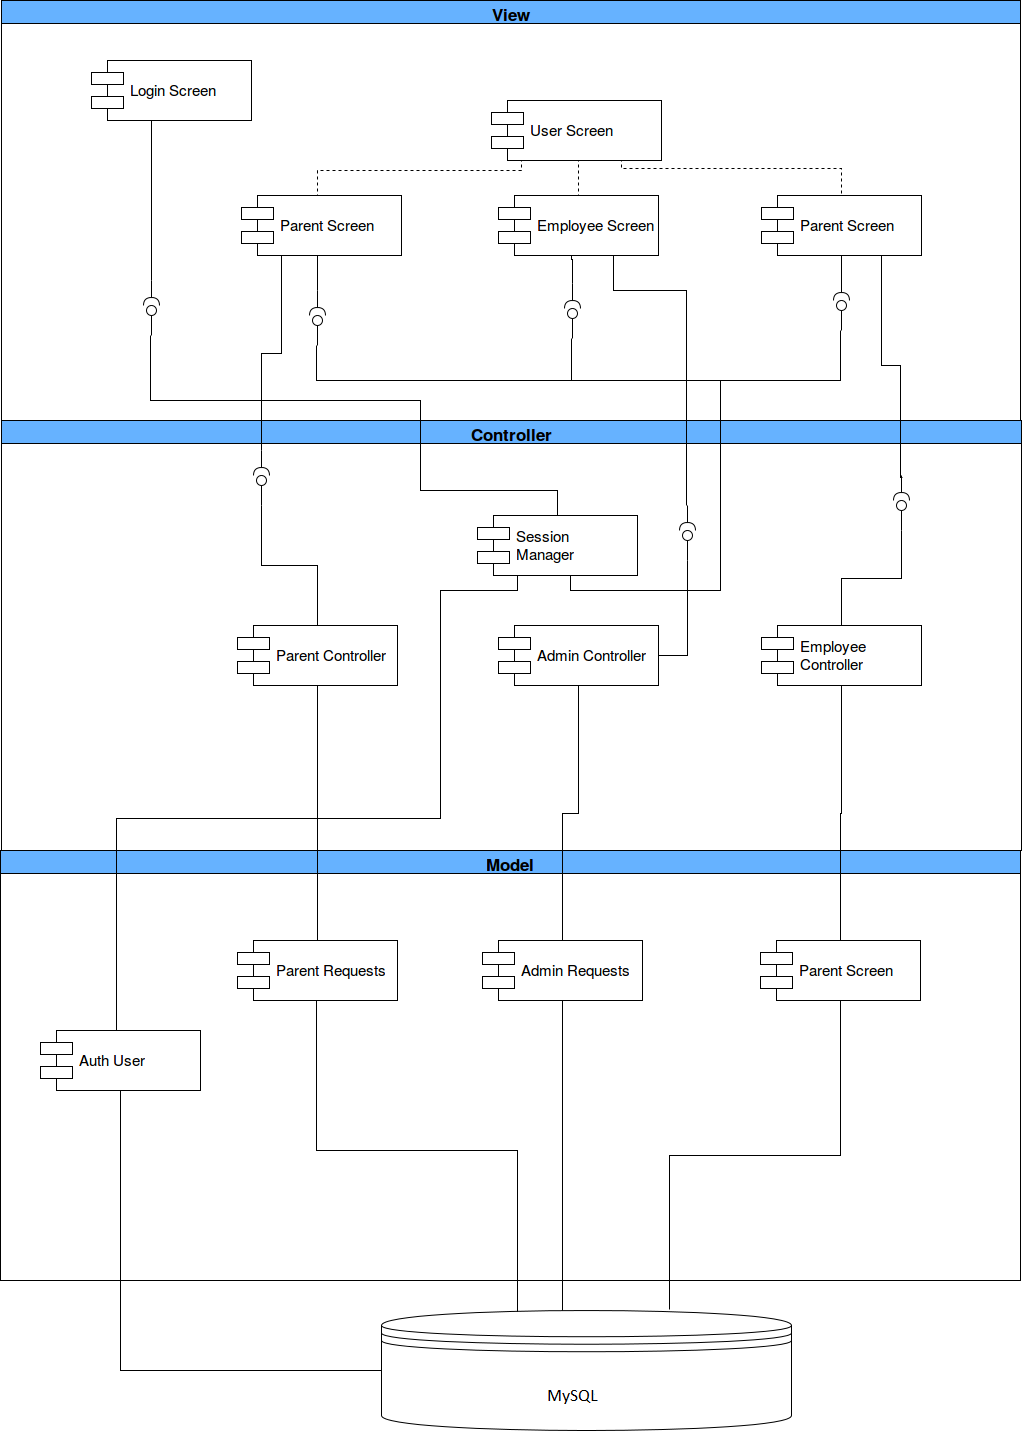
\includegraphics[scale=0.4]{component/Komponentendiagramm.png}
\end{figure}

\newpage
\section{GUI-Prototypen}
Im Grunde besteht das Projekt aus zwei grundlegenden Prototypen. Der Loginseite und der Templateseite f"ur alle weiteren Seiten. 
Die Templateseite unterscheidet sich minimal bei den unterschiedlichen Akteuren durch ihre Funktionalit"at.

\subsection{Loginseite}
 \begin{figure}[ht!]
  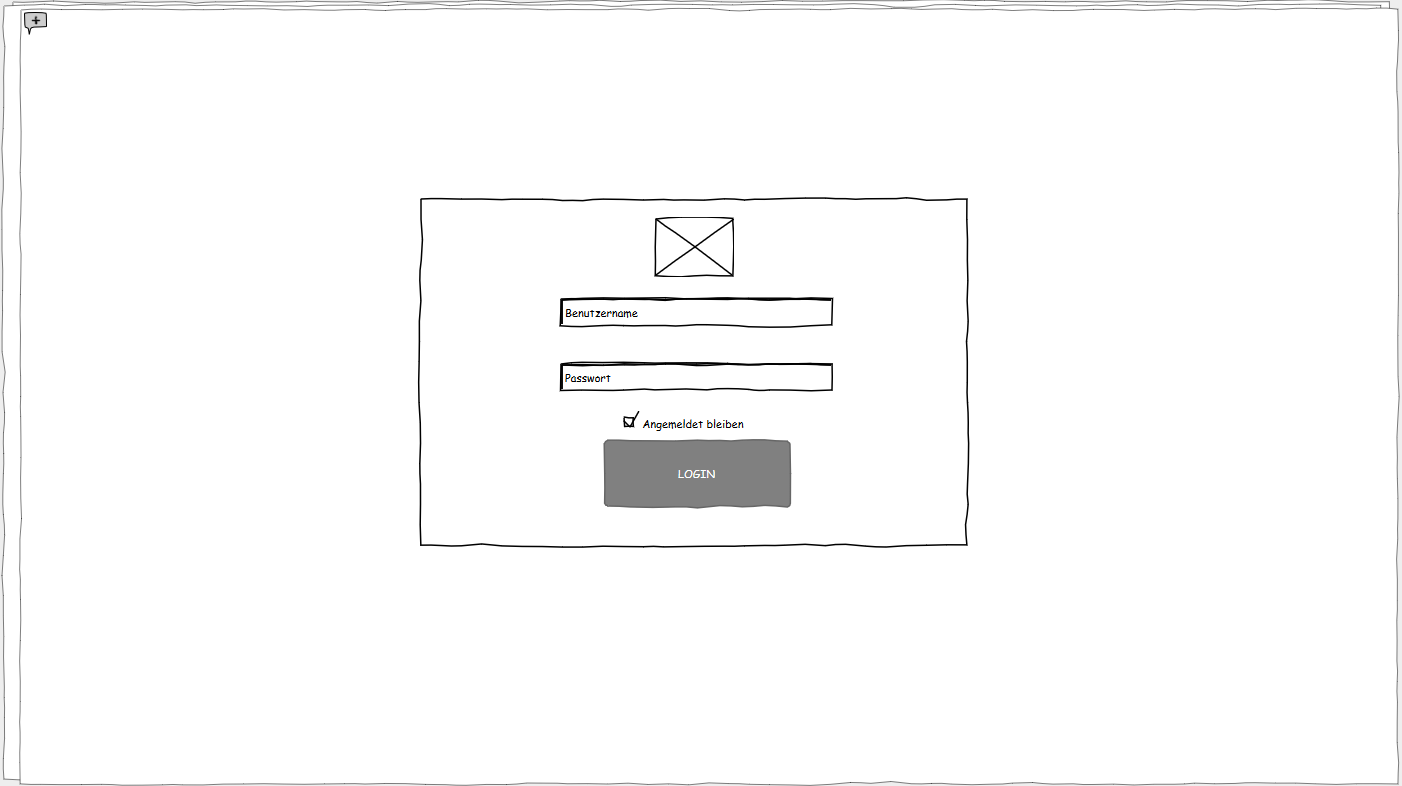
\includegraphics[width = 150mm]{pictures/Login.PNG}
 \end{figure}
 
 \newpage
 \subsection{Templateseite Elternteil}
 \begin{figure}[ht!]
  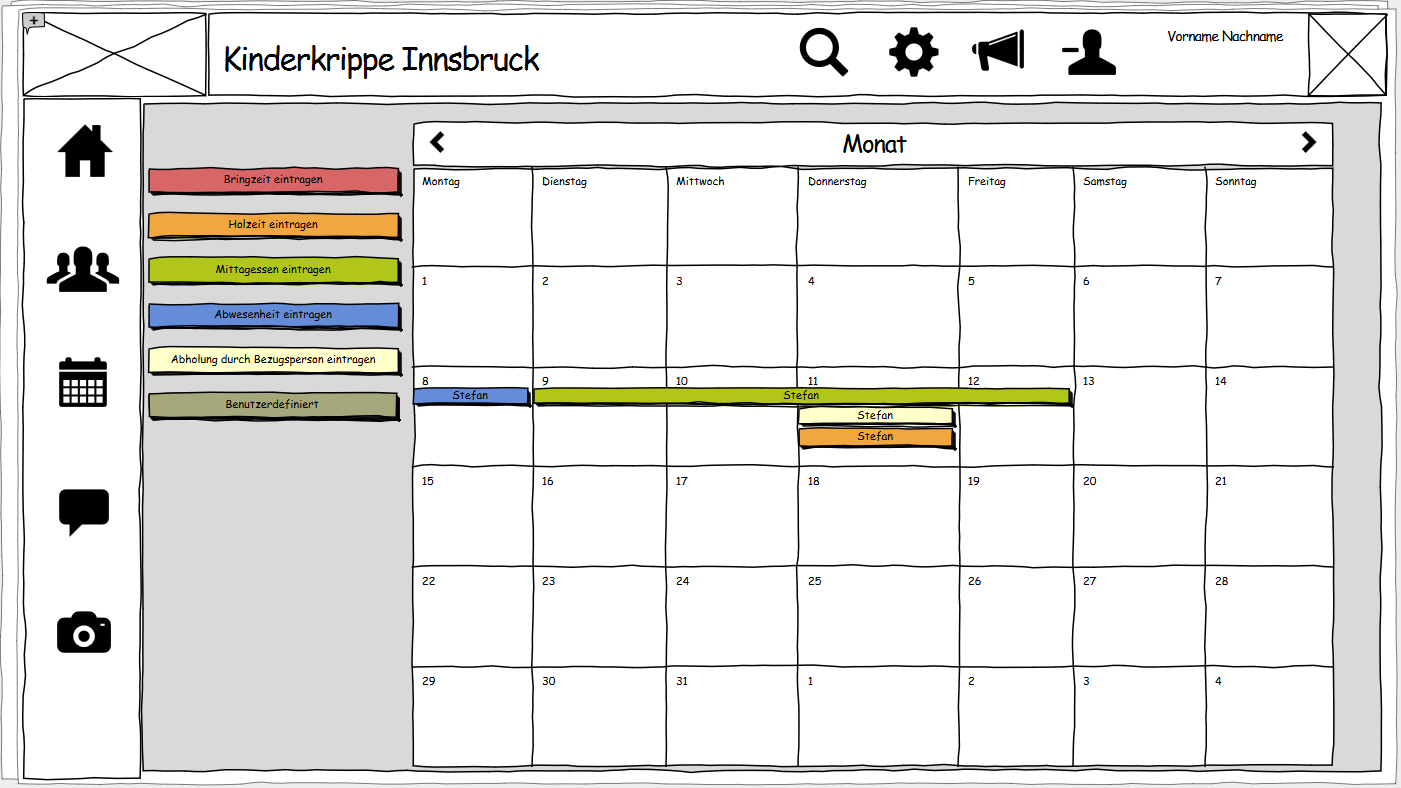
\includegraphics[width = 150mm]{pictures/Grundstellung_Elternteil.PNG}
 \end{figure}
 
  \subsection{Templateseite Mitarbeiter}
 \begin{figure}[ht!]
  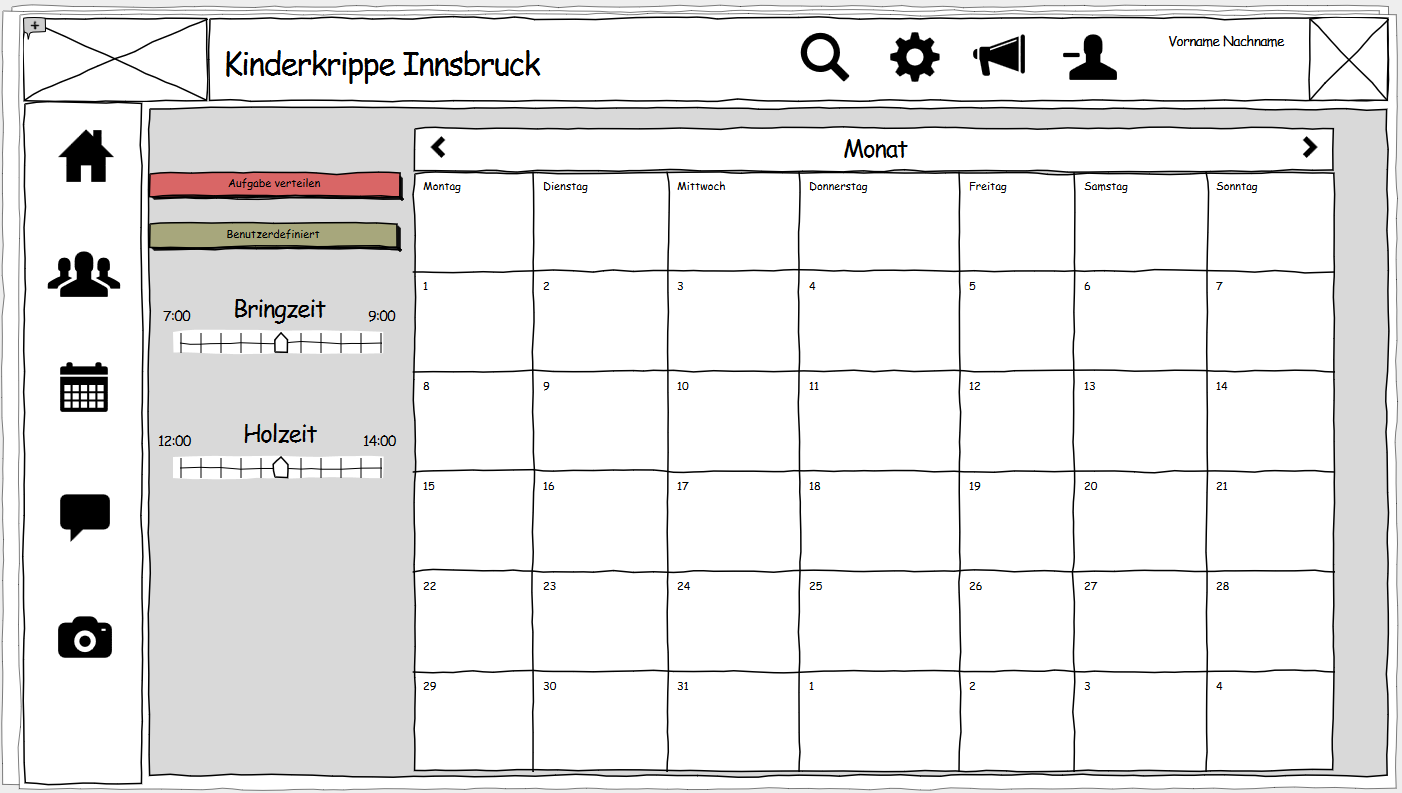
\includegraphics[width = 150mm]{pictures/Grundstellung_Mitarbeiter.PNG}
 \end{figure}
 
  \newpage
 \subsection{Templateseite Kontaktliste}
 \begin{figure}[ht!]
  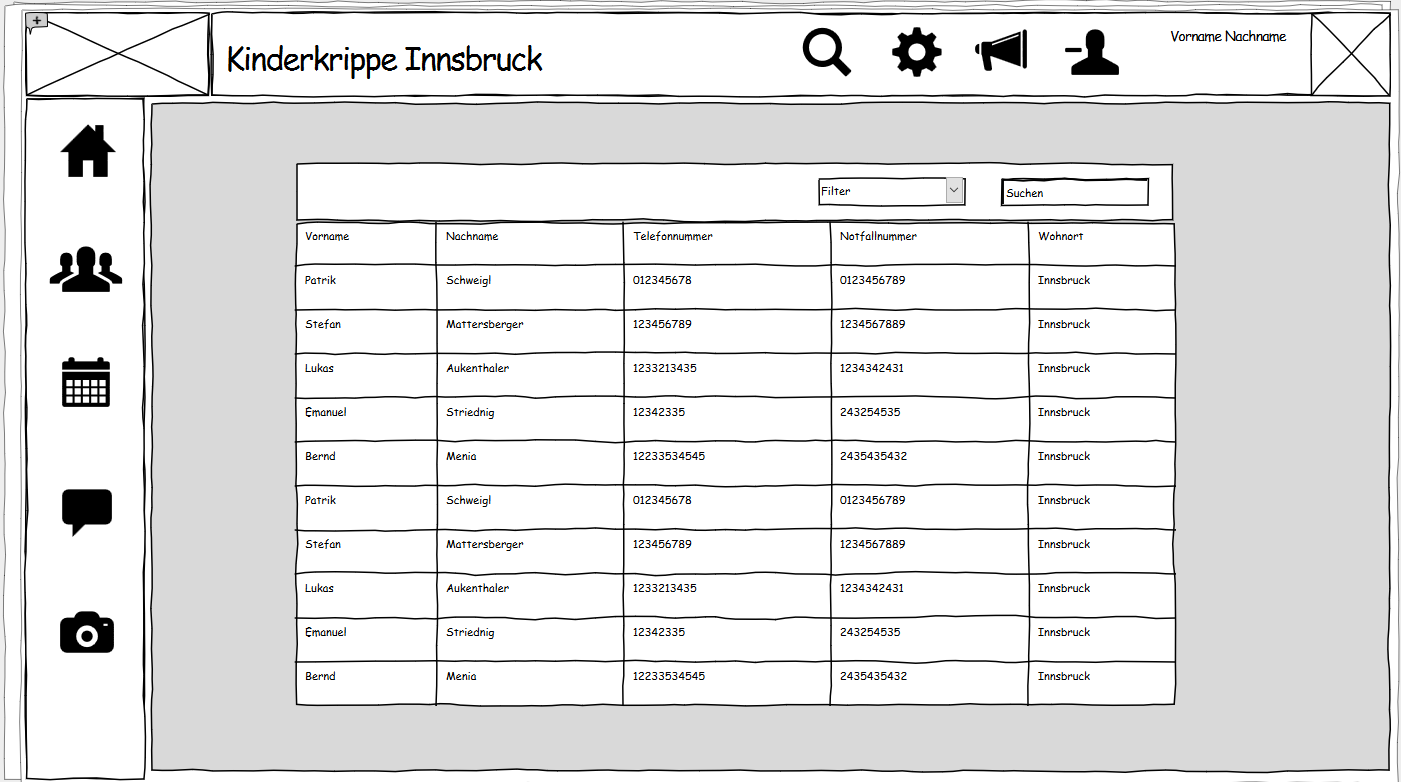
\includegraphics[width = 150mm]{pictures/Kontaktliste.PNG}
 \end{figure}
 
  \subsection{Templateseite Daten bearbeiten}
 \begin{figure}[ht!]
  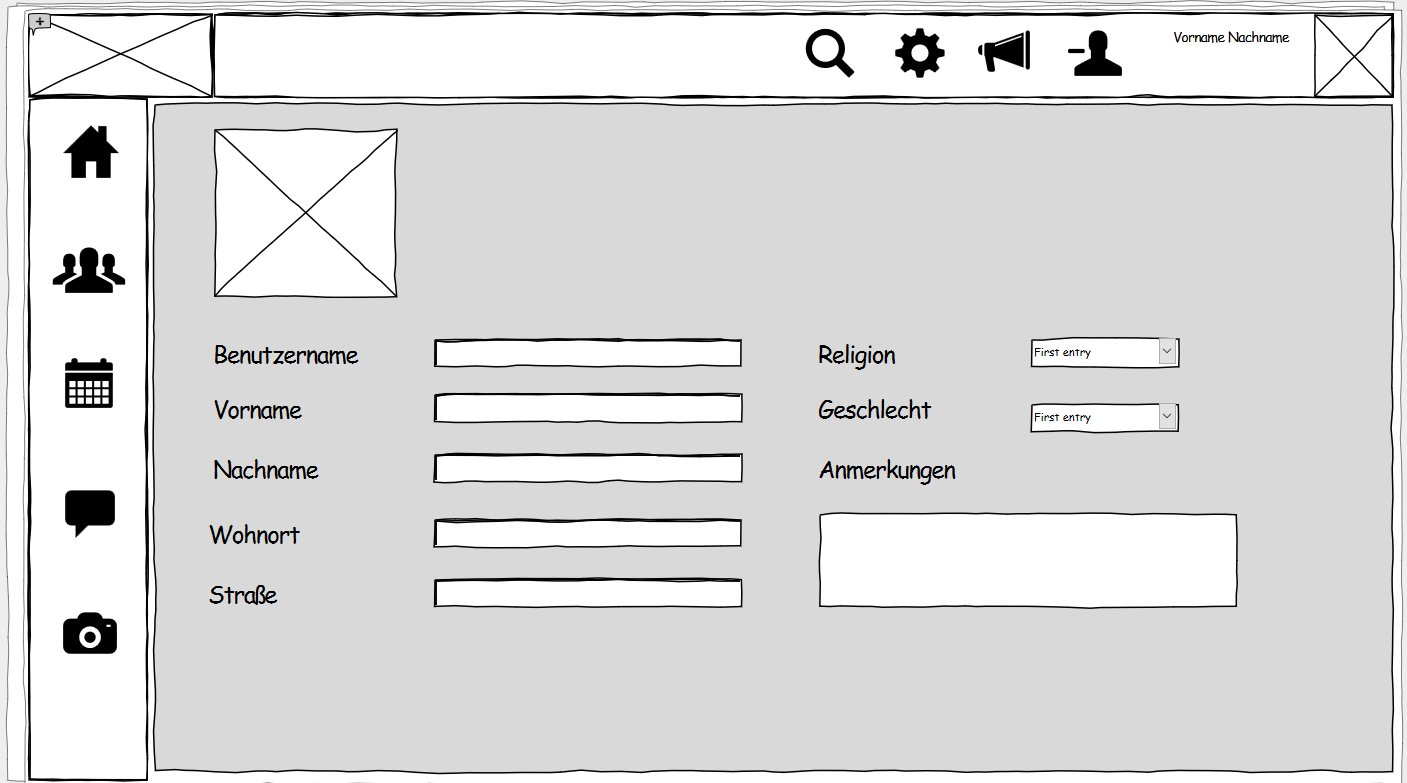
\includegraphics[width = 150mm]{pictures/daten_bearbeiten.PNG}
 \end{figure}
 
  \newpage
 \subsection{Templateseite Stammblatt}
 \begin{figure}[ht!]
  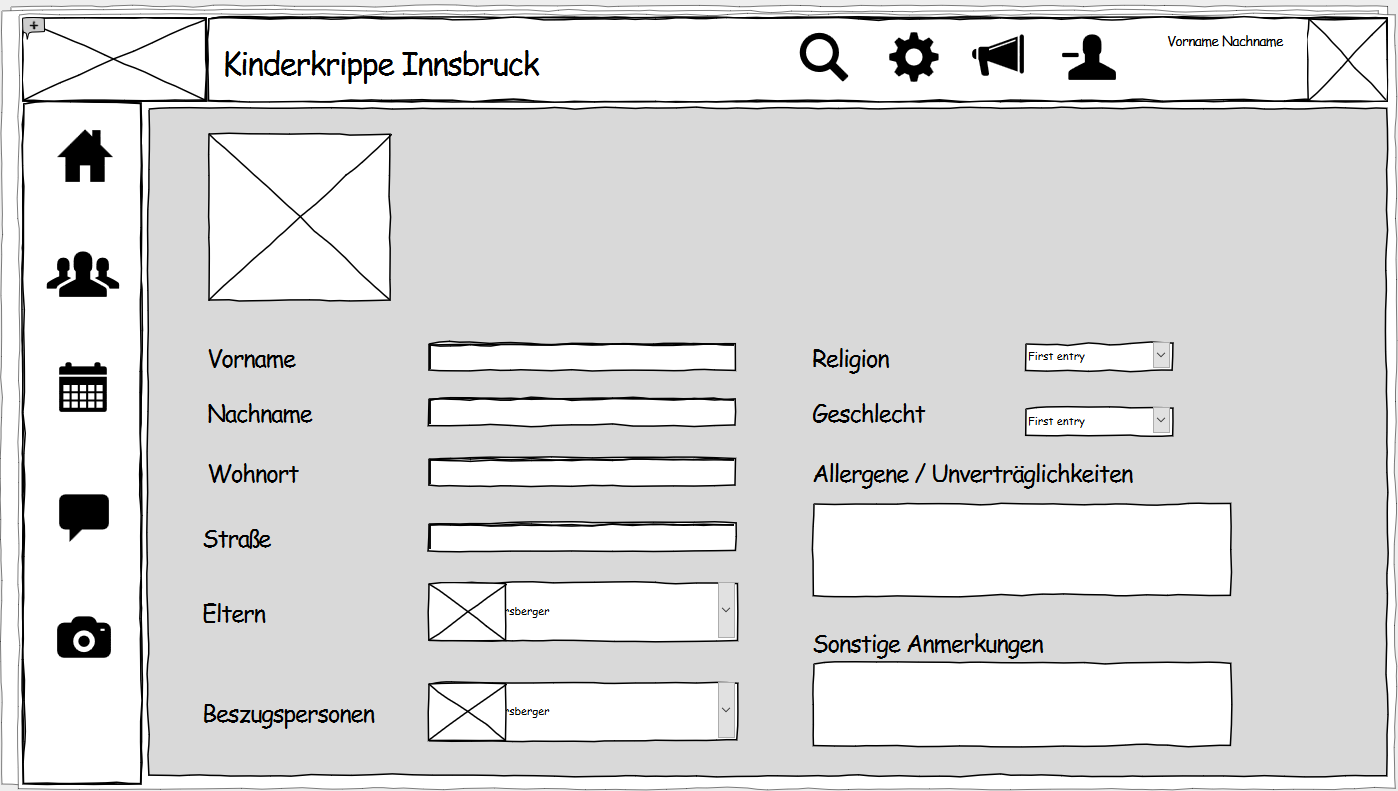
\includegraphics[width = 150mm]{pictures/Stammblattseite.PNG}
 \end{figure}
 
  \subsection{Templateseite Tagesplaner}
 \begin{figure}[ht!]
  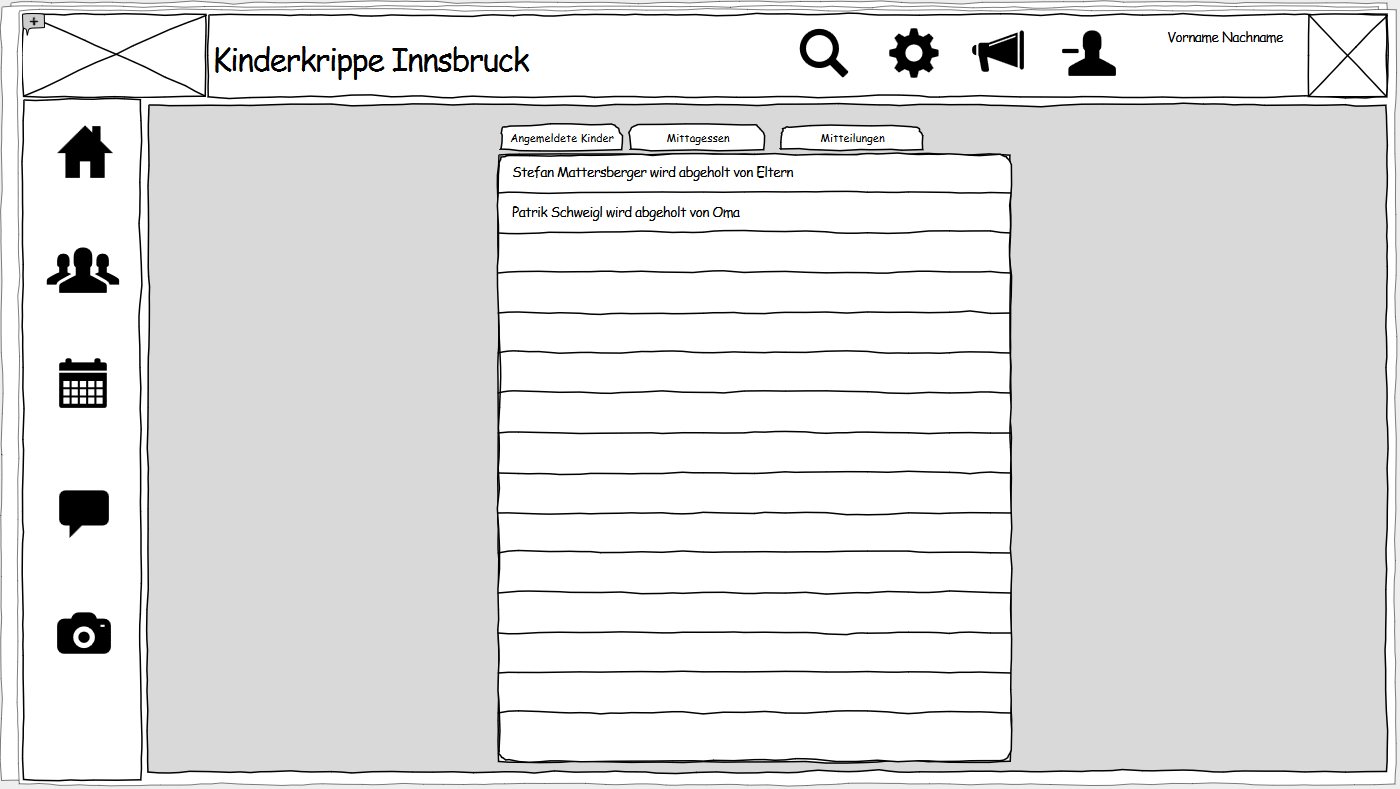
\includegraphics[width = 150mm]{pictures/Tagesplaner.PNG}
 \end{figure}
 
  \newpage
 \subsection{Templateseite Messageboard}
 \begin{figure}[ht!]
  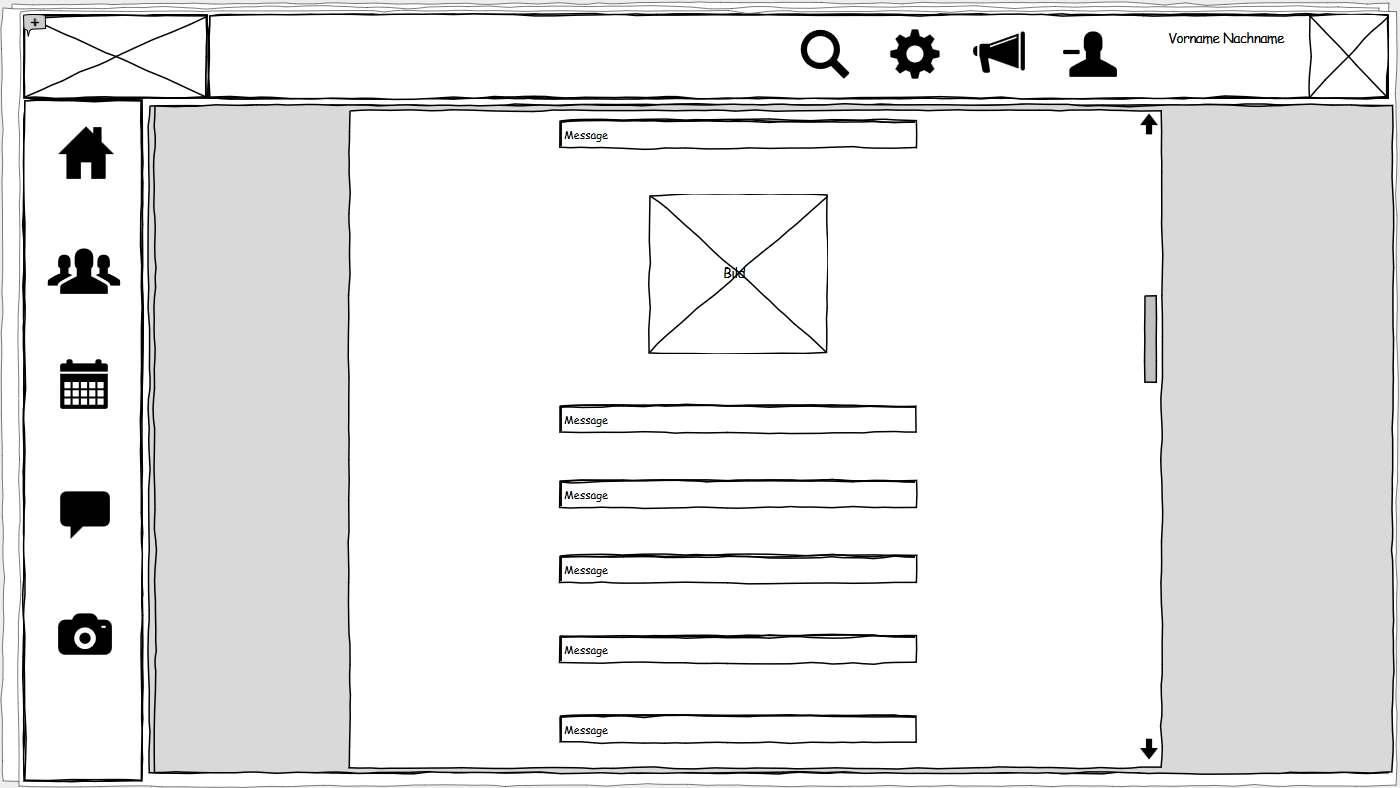
\includegraphics[width = 150mm]{pictures/Messageboard.PNG}
 \end{figure}
 
  \subsection{Templateseite Auditlog}
 \begin{figure}[ht!]
  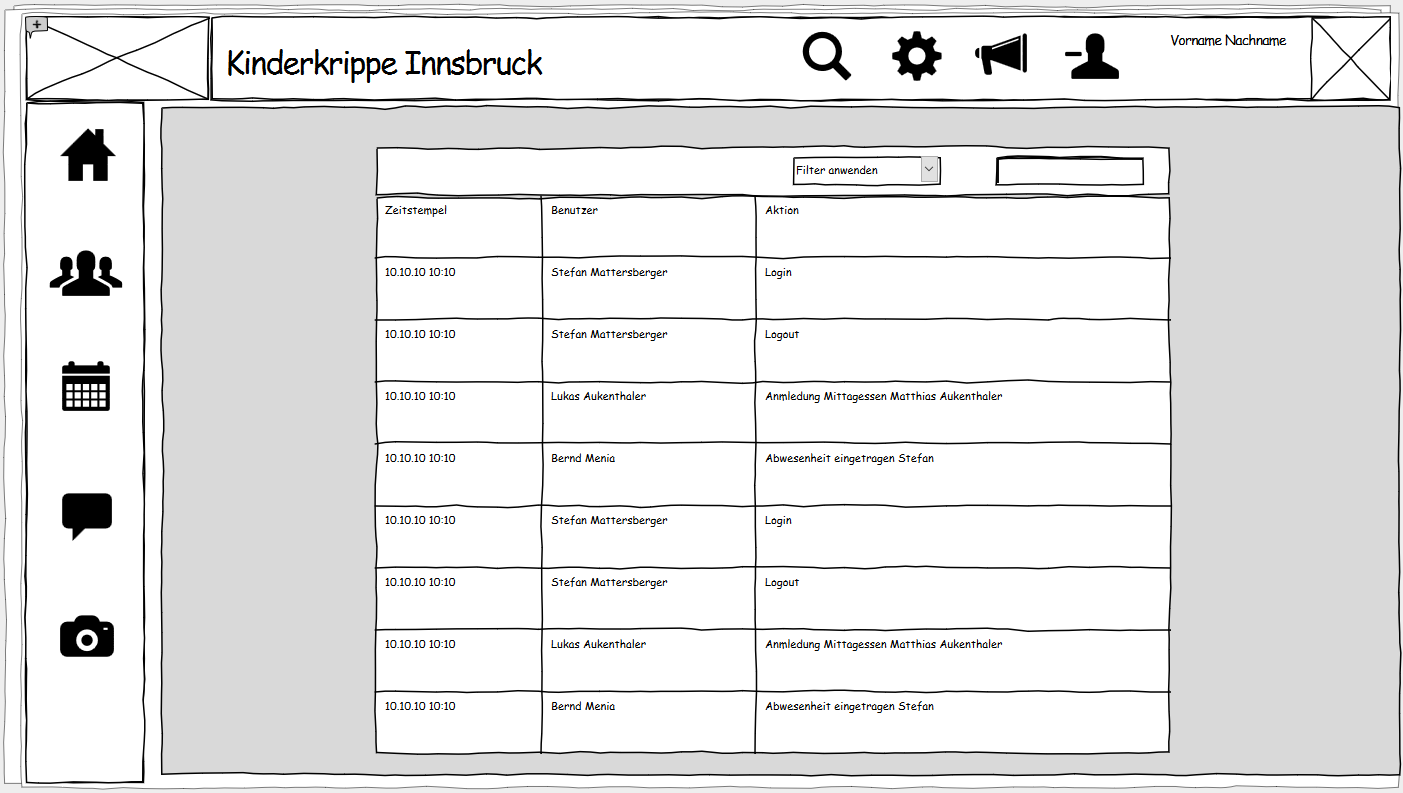
\includegraphics[width = 150mm]{pictures/Auditlog.PNG}
 \end{figure}
 
  \newpage
 \subsection{Templateseite Bildergalerie}
 \begin{figure}[ht!]
  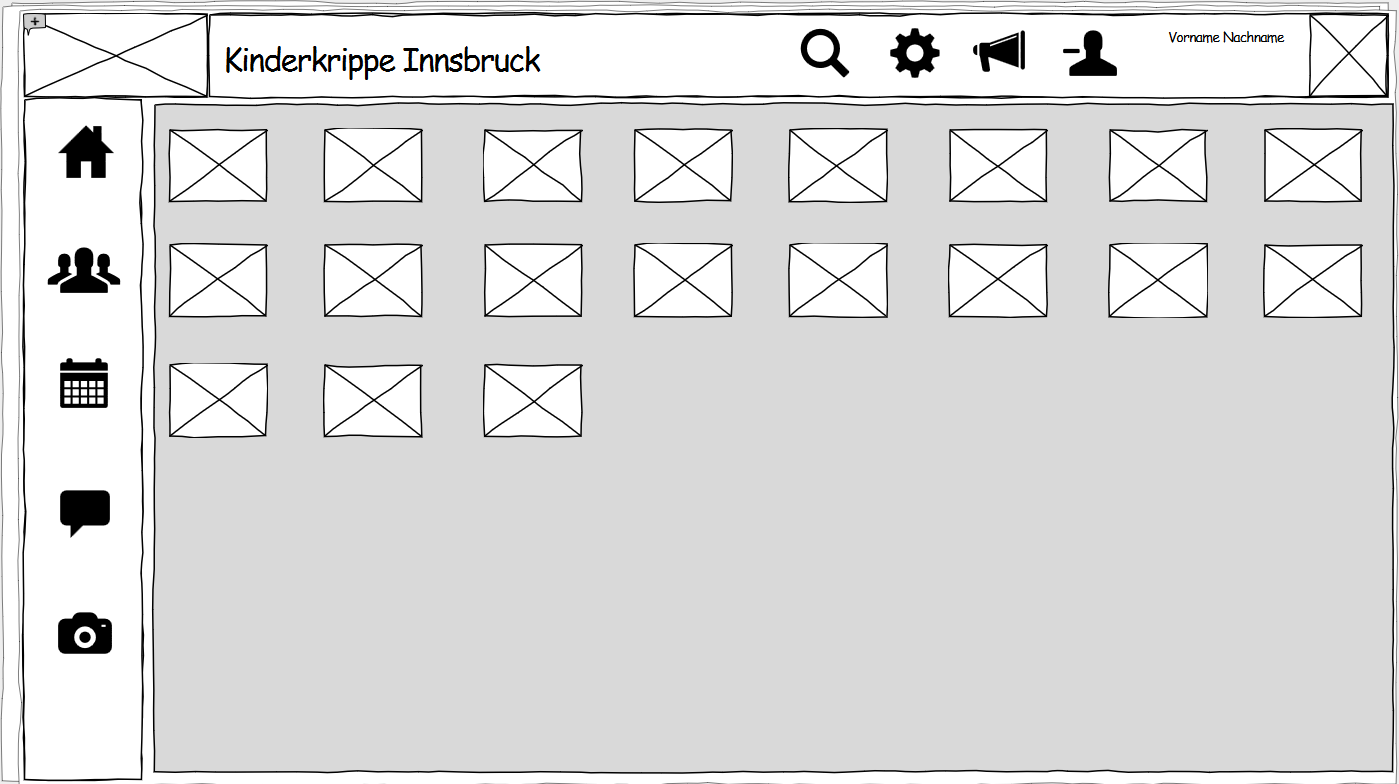
\includegraphics[width = 150mm]{pictures/Bildergalerie.PNG}
 \end{figure}
 
  \subsection{Templateseite Bildergalerie Detail}
 \begin{figure}[ht!]
  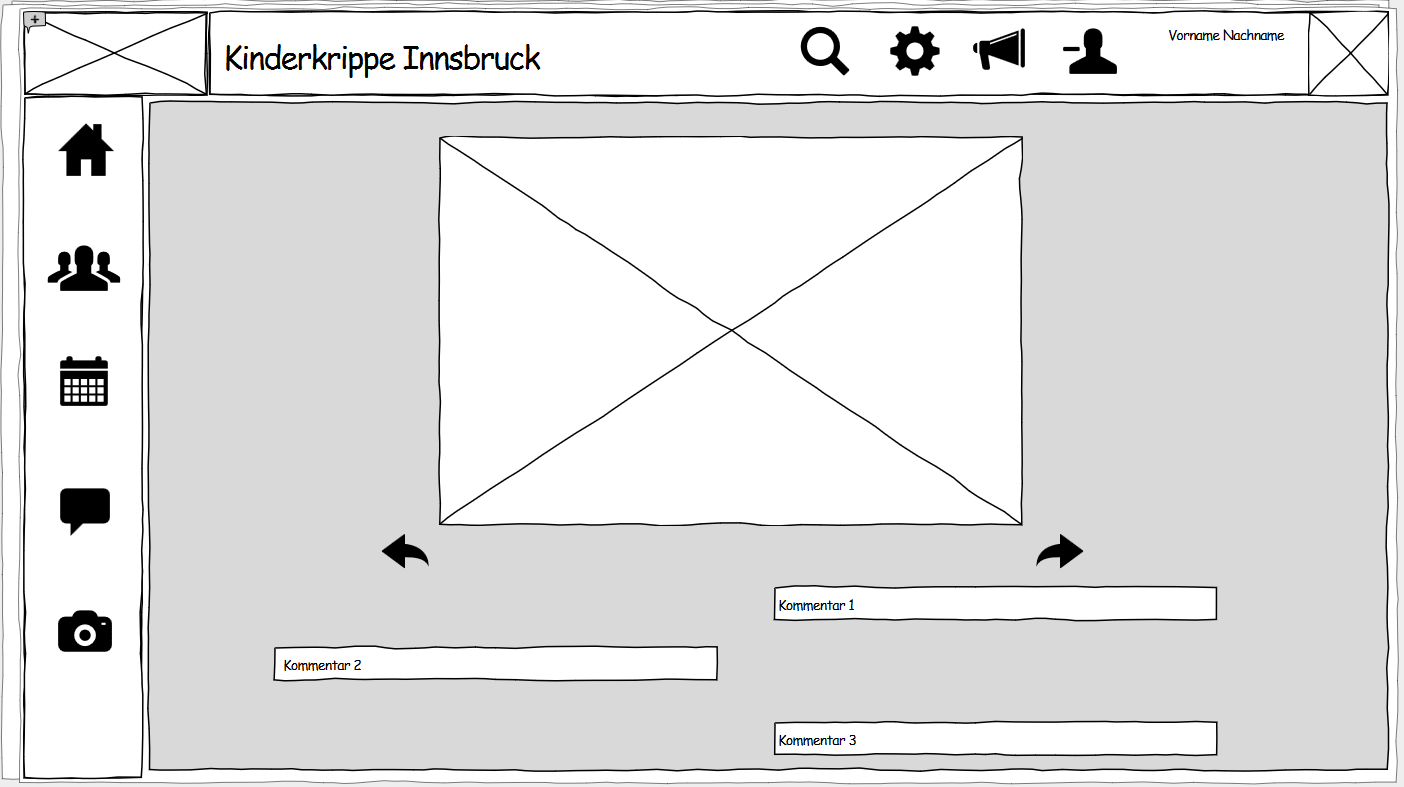
\includegraphics[width = 150mm]{pictures/Bildergalerie_detail.PNG}
 \end{figure}
 

\newpage
\section{Projektplan}
\subsection{Arbeitsaufteilung}
\paragraph{Datenbankmodellierung}
Stefan Mattersberger, Emanuel Striednig
\paragraph{Konzept}
Aukenthaler Lukas, Stefan Mattersberger, Bernd Menia, Patrik Schweigl, Emanuel Striednig
\paragraph{GUI}
Bernd Menia, Patrik Schweigl, Emanuel Striednig
\paragraph{Implementierung Use-Cases Benutzer}
Aukenthaler Lukas
\paragraph{Implementierung Use-Cases aktiver Benutzer}
Bernd Menia, Patrik Schweigl
\paragraph{Implementierung Use-Case Angestellter}
Stefan Mattersberger, Emanuel Striednig
\paragraph{Implementierung Sonderfeature}
Aukenthaler Lukas, Stefan Mattersberger, Bernd Menia, Patrik Schweigl, Emanuel Striednig
\paragraph{Tests}
Aukenthaler Lukas, Stefan Mattersberger, Bernd Menia, Patrik Schweigl, Emanuel Striednig
\newpage
\subsection{Meilensteine}
 \begin{figure}[ht!]
  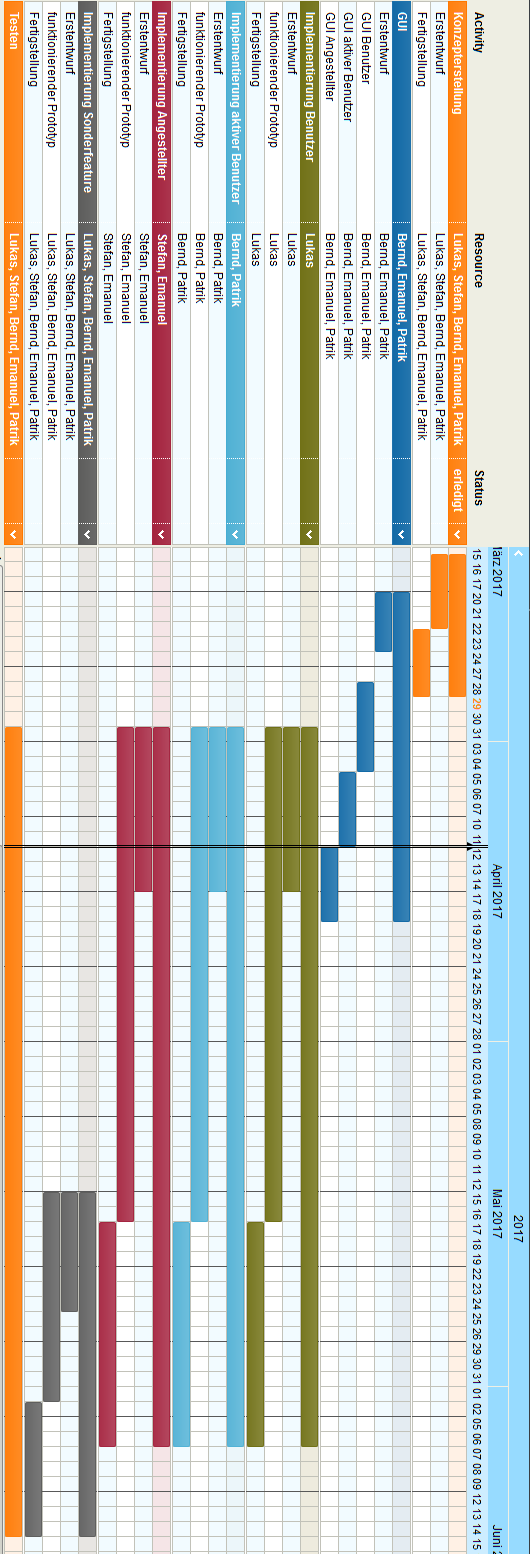
\includegraphics[width = 68mm]{pictures/Zeitplanneu.PNG}
 \end{figure}
\newpage
\pagenumbering{Roman}
\setcounter{page}{\value{roemisch}}

\appendix
%\input{extras/anhang}

\end{document}